We construct a graph $\mathcal{G}$ from the set of instances $\mathcal{X}$, where each data instance is a vertex and the edges represent the relationship between vertices. A model builds on this graph, combines with the information of labeled vertices to estimate the label for unlabeled vertices. In semi-supervised learning, the inferences that utilize the graph structure like this are called graph-based methods.

As an application of graph-based methods, in this chapter, we consider our data assumption in the form of an objective function on $\mathcal{G}$. Then the inference process aims to recognize the boundary between groups of different label vertices.

%The conventional approach solves this function and assigns the label for unlabeled vertices by finding a minimum cut on the graph. Nevertheless, the minimum cut frequently gives an unbalanced assignment when there is more than one solution. The thesis employs the idea of deriving a graphical model on this graph to bypass this problem. Furthermore, the affordable inference on graphical model only works with tree-like graph. Then an approximate algorithm is utilized to deal with the case when our graph does not have the tree form.

%%%%%
\section{Graph Construction}
\label{section3: Graph Construction}

Basically most graph-based methods are transductive learning. A common graph-based setup consists of two basic steps. The first is graph construction where the data is mapped to a graph, $\mathcal{X} \rightarrow \mathcal{G}$. Then in graph inference, we estimate labels for unlabeled data, $\{ \mathcal{G}, \mathcal{Y}_L \} \rightarrow \mathcal{Y}_U$.

In this chapter, we discuss the first step of graph construction. Denote that $n$ is the total number of instances, $n \triangleq l + u$. We initialize a graph $\mathcal{G} = (V, E, W)$, where $V=\{1,  ..., n\}$ is the set of vertices; $E \subseteq V \times V$ is the set of edges and $W$ is a $n \times n$ weight matrix on $E$. First, we need to establish and clarify the basic conditions on $\mathcal{G}$
\begin{description}
	\item[$\mathcal{G}$ is a simple weighted graph:] $\mathcal{G}$ does not contain self-loop and multiple edges; each edge is undirected and assigned with a weight value.
	
	\item[$V$ is constructed from data instances: ] $V$ is constructed by an one-to-one correspondence with data instances and its label, $\{ (\mathcal{X}, \mathcal{Y}) \} \rightarrow V$. This means each vertex contains information of an instance and its corresponding label. In practice, $\mathcal{Y}_U$ is initialized as non-clarified labels $\mathcal{Y}_U = \{ 0 \}^u$.
	
	\item[$W$ is positive and symmetric: ] $W \in \mathbb{R}^{n\times n}, W > 0$ and $W_{i,j} = W_{j,i}$. If $W_{i,j} = 0$ that means there is no edge between $i$ and $j$. In this thesis, we consider the weight on an edge between two vertices as the similarity between them. In other words, the larger the weight is, the more similar the two vertices.
\end{description}

Because the set of vertices $V$ is fixed, the remaining task involves estimating $E$ and $W$. Actually we only take into account the estimation of $W$, because it entirely defines the setup of $E$.

Typically the graph construction process contains two smaller steps: graph sparsification and graph re-weighting. Denote a similarity measure $S: V\times V \rightarrow \mathbb{R}^{n\times n}$ is a function that returns the similarity between two vertices. From the beginning, we initialize $\mathcal{G}$ as a fully connected graph $W_{i,j} = S(x^{(i)}, x^{(j)})$. In graph sparsification, we intend to sparsify $W$ through a binary mass matrix $P \in \{0, 1\}^{n\times n}$, where $P_{i,j} = 1$ means there is an edge between $i$ and $j$ and $0$ otherwise, start with $P$ of all zeros. There are many sparsification algorithms, though we only discuss the primary two that will be set in our practice
\begin{description}
	\item[K-nearest neighbors (kNN):] The typical kNN sparsification searches for the $k$ most similar vertices of each vertex. We set $P_{i,j} = 1$ if $j$ is one of the most similar neighbors of $i$. Also, if $i$ is a selected neighbor of $j$, then the reverse state does not hold. Thus to meet the symmetry condition of $W$, after searching, we have to re-symmetrize $P = max(P, P^T)$. This may lead to the misconception of the result kNN graph when after all we have $\sum_{j}{P_{i,j}} \geq k$, which means the graph would have more edges than expected.
	
	 \item[Maximum spanning tree (MST):] In this construction, we look for a spanning tree -- a tree containing all the vertices in $\mathcal{G}$, that has the highest sum of weights. We may further expand this structure by executing the MST on each component of the kNN graph. The benefit of this construction comes from its spanning tree structure, where we always receive the graph with a fixed number of $(n-1)$ edges. But this might be a trade-off if the graph is sparse, it could cause the lost information of vertices connection.
\end{description}

Continuing with the graph re-weighting, from the solution matrix $P$, we continue to re-estimate the weight of the selected edges to produce the final matrix $W$. The motivation of this task is to focus on some target characteristics that we aim at inference step and try to omit the misbehavior of $P$ from sparsification step. There are also some possible approaches to this task \parencite{Jebara:2009:GCB:1553374.1553432, Subramanya:2014:GSL:2765801}. For simplification purposes, we utilize the simplest schedule using the element-wise product to set $W = W \cdot P$. The graph construction process is summarized in algorithm \ref{alg4: graph construction}. It takes the instances set $\mathcal{X}$, label of labeled instances $\mathcal{Y}_L$ and similarity measure $S$ as input and outputs the graph as a pair of vertices set and weight matrix $(V, W)$.
\begin{algorithm}[H]
	\caption{Graph construction process}
	\begin{algorithmic}[1]
		\Function{Graph\_Construction}{$\mathcal{X}, \mathcal{Y}_L, S$}
		
		\State $\mathcal{Y}_U \gets \{0\}^u$
		\COMMENT{Initialize label for unlabeled instances}
		\State $\mathcal{Y} \gets \mathcal{Y}_L \cup \mathcal{Y}_U$
		\COMMENT{Merge the complete label sets}
		\State $V \gets \{(\mathcal{X}, \mathcal{Y})\}$
		\COMMENT{Set $V$ as set of (instance, label)}
		
		\State $W \gets S(V \times V)$
		\COMMENT{Initialize $W$ by similarity measure $S$}
		\State $P = Sparsify(W)$
		\COMMENT{Sparsify $W$}
		\State $W \gets W \cdot P$
		\COMMENT{Re-weigh $W$}
		\RETURN $(V, W)$
		
		\EndFunction
	\end{algorithmic}
	\label{alg4: graph construction}
\end{algorithm}

So far we have been constructing the graph. In the next section we will discuss how to inferring the labels for unlabeled vertices.

%%%%%
\section{Minimum Cut Inference}
\label{section3: mincut approach}

Given our graph after construction $\mathcal{G}$. We presume that the vertices set $V$ is the union of $V_L$ and $V_U$ respectively are the subsets of labeled and unlabeled vertices,  $V = V_L \cup V_U$. Moreover, we assume $U_L = U_{L^+} \cup U_{L^-}$, where $U_{L^+}$ is the positive vertices set and $U_{L^-}$ is the negative vertices set of labeled vertices. We construct a simple target function
\begin{align}
\label{equal4: target function}
\argmin_{f} \quad \frac{1}{2}\sum_{(i,j) \in E}{W_{i,j}|f(i) - f(j)|}
\end{align}
where $f(i) \in \{-1, +1\}$ represents labels for $i \in V$. With $i \in V_L$, $f(i) = -1$ if $i \in U_{L^-}$ and otherwise, $f(i) = +1$ if $i \in U_{L^+}$.

Now let's consider the intuition viewing of  (\ref{equal4: target function}). In \parencite{Blum:2001:LLU:645530.757779}, we have an interesting expression of our implied generative framework in there. We assume that the underlying distribution is a fixed number of combined components---groups of vertices---and each has a unique label. Components are separated by a minimum dissimilarity value. An instance is generated by randomly picking a vertex in one of these components then giving it the label of component which it belongs to. 

The hypothesis here is that with proper graph construction, there is a sparse connection between two components and more densely connected edges inside oneself. Then with a large enough unlabeled data, the component will be more dense and the connection between them will be the loosest one. So they become the boundary to separate the components. Thus, with only a few labeled vertices on each component, we can label all of them. Figure \ref{fig4: combination of components assumption} gives an illustration for these views with four regions of positive and negative labels.
\begin{figure}[!ht]
	\centering
	\begin{subfigure}[b]{0.4\textwidth}
		\centering
		\begin{tikzpicture}[
		scale=.7, auto,swap,
		declare function={a1(\x)=(1 - \x^2)^0.5 - 2;},
		declare function={a2(\x)= -(1 - \x^2)^0.5 - 2;},
		declare function={b1(\x)=(1 - \x^2)^0.5 + 2;},
		declare function={b2(\x)= -(1 - \x^2)^0.5 + 2;},
		declare function={c1(\x)= (1 - (\x + 2)^2)^0.5;},
		declare function={c2(\x)= -(1 - (\x + 2)^2)^0.5;},
		declare function={d1(\x)= (1 - ((\x - 3)^2)/3)^0.5;},
		declare function={d2(\x)= -(1 - ((\x - 3)^2)/3)^0.5;}
		]
		\pgfmathsetseed{1355}
		\begin{axis}[
		% axis line style={draw=none},
		xtick=\empty, ytick=\empty
		]
		\addplot [positive data, samples=5]
		{0.5*(a1(x)+a2(x)) + 0.5*rand*(a1(x)-a2(x))};
		\addplot [positive data, samples=5]
		{0.5*(d1(x)+d2(x)) + 0.5*rand*(d1(x)-d2(x))};
		\addplot [unlabeled data, samples=60]
		{0.5*(a1(x)+a2(x)) + 0.5*rand*(a1(x)-a2(x))};
		\addplot [unlabeled data, samples=60]
		{0.5*(d1(x)+d2(x)) + 0.5*rand*(d1(x)-d2(x))};
		
		\addplot [negative data, samples=5]
		{0.5*(b1(x)+b2(x)) + 0.5*rand*(b1(x)-b2(x))};
		\addplot [negative data, samples=5]
		{0.5*(c1(x)+c2(x)) + 0.5*rand*(c1(x)-c2(x))};
		\addplot [unlabeled data, samples=60]
		{0.5*(b1(x)+b2(x)) + 0.5*rand*(b1(x)-b2(x))};
		\addplot [unlabeled data, samples=60]
		{0.5*(c1(x)+c2(x)) + 0.5*rand*(c1(x)-c2(x))};
		\end{axis}
		\end{tikzpicture}
		\caption{}
		\label{fig4.a: combination of components assumption}
	\end{subfigure}
	\begin{subfigure}[b]{0.4\textwidth}
		\centering
		\begin{tikzpicture}[
		scale=.7, auto,swap,
		declare function={a1(\x)=(1 - \x^2)^0.5 - 2;},
		declare function={a2(\x)= -(1 - \x^2)^0.5 - 2;},
		declare function={b1(\x)=(1 - \x^2)^0.5 + 2;},
		declare function={b2(\x)= -(1 - \x^2)^0.5 + 2;},
		declare function={c1(\x)= (1 - (\x + 2)^2)^0.5;},
		declare function={c2(\x)= -(1 - (\x + 2)^2)^0.5;},
		declare function={d1(\x)= (1 - ((\x - 3)^2)/3)^0.5;},
		declare function={d2(\x)= -(1 - ((\x - 3)^2)/3)^0.5;}
		]
		\pgfmathsetseed{1355}
		\begin{axis}[
%		 axis line style={draw=none},
		xtick=\empty, ytick=\empty
		]
		\addplot [positive data, samples=5]
		{0.5*(a1(x)+a2(x)) + 0.5*rand*(a1(x)-a2(x))};
		\addplot [positive data, samples=5]
		{0.5*(d1(x)+d2(x)) + 0.5*rand*(d1(x)-d2(x))};
		\addplot [positive data, samples=60, style=semithick]
		{0.5*(a1(x)+a2(x)) + 0.5*rand*(a1(x)-a2(x))};
		\addplot [positive data, samples=60, style=semithick]
		{0.5*(d1(x)+d2(x)) + 0.5*rand*(d1(x)-d2(x))};
		
		\addplot [negative data, samples=5]
		{0.5*(b1(x)+b2(x)) + 0.5*rand*(b1(x)-b2(x))};
		\addplot [negative data, samples=5]
		{0.5*(c1(x)+c2(x)) + 0.5*rand*(c1(x)-c2(x))};
		\addplot [negative data, samples=60, style=semithick]
		{0.5*(b1(x)+b2(x)) + 0.5*rand*(b1(x)-b2(x))};
		\addplot [negative data, samples=60, style=semithick]
		{0.5*(c1(x)+c2(x)) + 0.5*rand*(c1(x)-c2(x))};
		
		% bound
    	\addplot[mark=none] coordinates { (-3,-3) (4,3) } node [midway, sloped, above] {boundary};

		\end{axis}
		\end{tikzpicture}
		\caption{}
		\label{fig4.b: combination of components assumption}
	\end{subfigure}
	\hfill
	\caption[Illustration of the combination of components assumption.]{Illustration of the combination of components assumption. There are two positive regions and two negative regions. When there is enough unlabeled data, each component will form as a dense graph---figure (a). Thus, with only one labeled vertex on each component, we can decide the boundary and label all unlabeled vertices---figure (b).}
	\label{fig4: combination of components assumption}
\end{figure}

We are now looking for the inference which can be adapted to the optimization condition (\ref{equal4: target function}) above. Literally, the solution is a configuration of $f(i), i \in V_U$ that guarantees the minimization. With a small set of unlabeled data, a brute-force approach that finds all the $2^u$ configurations of unlabeled vertices seems like a possible solution. But the basic condition of semi-supervised learning is a large scale of $u$. A common solution for this inference is using a minimum cut on $\mathcal{G}$, the mincut approach \parencite{Blum:2001:LLU:645530.757779}. It finds a minimum cut on which it separates all positive and negative vertices. Recall a cut $C= \{C_1, C_2\}$ on $\mathcal{G}$ is a segmentation of $V$ such that $C_1 \cap C_2 = \emptyset, C_1 \cup C_2 = V$. The size of cut $C$ is the total weight of edges between $C_1$ and $C_2$. More precisely, denote $W_C$ is the size of the cut, we have $W_C = \sum_{i \in C_1, j \in C_2} W_{i,j}$. Given a pair of source and sink vertices $(s, t)$, the minimum cut algorithm finds a cut with smallest weight such that $s \in C_1$ and $t \in C_2$. The solution for finding minimum cut is a well-known algorithm in graph theory and can be archived in polynomial running time. The detailed descriptions and tutorials of this algorithm can be found in \parencite{cormen2009introduction, West2001}.

Define that $MinCut(\mathcal{G}, s, t)$ is a function which is searching for a minimum cut on $\mathcal{G}$ with source vertex $t$ and sink vertex $s$. The output returns a cut $C$ with $s \in C_1$ and $t \in C_2$. The mincut approach starts by adding two new pseudo vertices $v_+$ and $v_-$ to $V$, then connects $v_+$ with all positive vertices and $v_-$ with all negative vertices. These pseudo vertices are treated as the stakes that keep all positive and negative vertices in separate parts. When we have a minimum cut on $\mathcal{G}$ with $v_+$ and $v_-$ are source and sink, MinCut$(\mathcal{G}, v_+, v_-)$, we can label all unlabeled vertices using its correspondence with $v_+$ or $v_-$. All vertices in the part containing $v_+$ will have the positive label and all vertices in the part of $v_-$ will have the negative label. Figure \ref{fig4: mincut example} illustrates the process of mincut approach and we summarize the process in algorithm \ref{alg4: mincut}. It receives the graph $\mathcal{G}$ as input and returns the vertices set $V$ after labeling all unlabeled vertices.

It is obvious that the complexity of this approach mainly comes from the function MinCut$(\mathcal{G}, s, t)$. Constantly, the problem of finding a minimum s-t cut in graph is similar to looking for a maximum flow on $\mathcal{G}$. For quick implementation, we may take the well known Edmonds–Karp algorithm \parencite{Edmonds:1972:TIA:321694.321699} which costs us $\mathcal{O}(n|E|^2)$ to find the solution. One of the more advanced methods, the push-relabel algorithm \parencite{KING1994447}, is commonly supported in difference graph frameworks having the complexity of $\mathcal{O}(n|E|\log{\frac{n^2}{|E|}})$. There are also other methods that would save more time, but they are far more complicated to be considered in our meaning time.

\begin{figure}[!ht]
	\centering
	\captionsetup[subfigure]{justification=centering}
	\begin{subfigure}[b]{0.4\textwidth}
		\centering
		\begin{tikzpicture}[scale=1.3, auto,swap]
		% First we draw the vertices
		\foreach \pos/\label/\name in {
			{(0,0)/a/+}, {(1,0)/b/}, {(2,0)/c/},
			{(0,1)/e/+}, {(1,1)/f/}, {(2,1)/g/}}
		\node[positive vertex] (\label) at \pos{$\name$};
		
		\foreach \pos/\label/\name in {{(3,0)/d/-}, {(3,1)/h/-}}
		\node[negative vertex] (\label) at \pos{$\name$};
		
		% Connect vertices with edges and draw weights
		\foreach \source/ \dest in {
			b/e,b/g,d/g}
		\path[thickedge] (\source) -- (\dest);
		\foreach \source/ \dest in {
			a/b,a/e,b/c,c/d,d/h,e/f,f/g,g/h}
		\path[edge] (\source) -- (\dest);
		\end{tikzpicture}
		\caption*{Input graph $G$, weight is represented as edge thickness.}
	\end{subfigure}
	\hfill
	\begin{subfigure}[b]{0.5\textwidth}
		\centering
		\begin{tikzpicture}[scale=1.3, auto,swap]
		% First we draw the vertices
		\foreach \pos/\label/\name in {
			{(0,0)/a/+}, {(1,0)/b/}, {(2,0)/c/},
			{(0,1)/e/+}, {(1,1)/f/}, {(2,1)/g/}, {(-1,0.5)/v+/v_+}}
		\node[positive vertex] (\label) at \pos{$\name$};
		
		\foreach \pos/\label/\name in {{(3,0)/d/-}, {(3,1)/h/-}, {(4,0.5)/v-/v_-}}
		\node[negative vertex] (\label) at \pos{$\name$};
		
		% Connect vertices with edges and draw weights
		\foreach \source/ \dest in {
			b/e,b/g,d/g}
		\path[thickedge] (\source) -- (\dest);
		\foreach \source/ \dest in {
			a/b,a/e,b/c,c/d,d/h,e/f,f/g,g/h}
		\path[edge] (\source) -- (\dest);
		
		% inf weight
		\path[draw, line width=3pt] (v+) -- node[sloped, above]{\footnotesize $\infty$} (e);
		\path[draw, line width=3pt] (v-) -- node[sloped, above]{\footnotesize $\infty$} (h);
		
		\path[draw, line width=3pt] (v+) -- node[sloped, below]{\footnotesize $\infty$} (a);
		\path[draw, line width=3pt] (v-) -- node[sloped, below]{\footnotesize $\infty$} (d);
		\end{tikzpicture}
		\caption*{Step 1, add pseudo vertices $v_+, v_-$ and corresponding edges.}
	\end{subfigure}

	\vspace*{5pt}
	\begin{subfigure}[b]{0.5\textwidth}
		\centering
		\begin{tikzpicture}[scale=1.3, auto,swap]
		% First we draw the vertices
		\foreach \pos/\label/\name in {
			{(0,0)/a/+}, {(1,0)/b/}, {(2,0)/c/},
			{(0,1)/e/+}, {(1,1)/f/}, {(2,1)/g/}, {(-1,0.5)/v+/v_+}}
		\node[positive vertex] (\label) at \pos{$\name$};
		
		\foreach \pos/\label/\name in {{(3,0)/d/-}, {(3,1)/h/-}, {(4,0.5)/v-/v_-}}
		\node[negative vertex] (\label) at \pos{$\name$};
		
		% Connect vertices with edges and draw weights
		\foreach \source/ \dest in {
			b/e,b/g,d/g}
		\path[thickedge] (\source) -- (\dest);
		\foreach \source/ \dest in {
			a/b,a/e,b/c,c/d,d/h,e/f,f/g,g/h}
		\path[edge] (\source) -- (\dest);
		
		% inf weight
		\path[draw, line width=3pt] (v+) -- node[sloped, above]{\footnotesize $\infty$} (e);
		\path[draw, line width=3pt] (v-) -- node[sloped, above]{\footnotesize $\infty$} (h);
		
		\path[draw, line width=3pt] (v+) -- node[sloped, below]{\footnotesize $\infty$} (a);
		\path[draw, line width=3pt] (v-) -- node[sloped, below]{\footnotesize $\infty$} (d);
		
		\path[dashedge] (1.5, 1.5) -- (1.5, -0.5);
		\end{tikzpicture}
		\caption*{Step 2, find a minimum cut in G with source $v_+$ and sink $v_-$.}
	\end{subfigure}
	\hfill
	\begin{subfigure}[b]{0.4\textwidth}
		\centering
		\begin{tikzpicture}[scale=1.3, auto,swap]
		% First we draw the vertices
		% First we draw the vertices
		\foreach \pos/\label/\name in {
			{(0,0)/a/+}, {(0,1)/e/+}, {(1,0)/b/+}, {(1,1)/f/+}}
		\node[positive vertex] (\label) at \pos{$\name$};
		
		\foreach \pos/\label/\name in {
			{(3,0)/d/-}, {(3,1)/h/-}, {(2,1)/g/-}, {(2,0)/c/-}}
		\node[negative vertex] (\label) at \pos{$\name$};
		
		% Connect vertices with edges and draw weights
		\foreach \source/ \dest in {
			b/e,b/g,d/g}
		\path[thickedge] (\source) -- (\dest);
		\foreach \source/ \dest in {
			a/b,a/e,b/c,c/d,d/h,e/f,f/g,g/h}
		\path[edge] (\source) -- (\dest);
		
		\path[dashedge] (1.5, 1.5) -- (1.5, -0.5);
		\end{tikzpicture}
		\caption*{Step 3, use this cut to label unlabeled vertices.}
	\end{subfigure}
	\caption{Example of mincut approach.}
	\label{fig4: mincut example}
\end{figure}

\begin{algorithm}[H]
	\caption{Semi-supervised mincut approach}
	\begin{algorithmic}[1]
		\Function{Mincut\_SSL}{$\mathcal{G}, s, t$}
		\State \texttt{\# Step 1}
		\State{$V \gets V \cup \{v_+, v_-\}$}
		\COMMENT{Add in $\mathcal{G}$ two new vertices $v_+$ and $v_-$}
		\For{$i \in V_{L^+}$}
		\COMMENT{For each positive vertices:}
		\State{$W_{i, v_+} \gets +\infty$}
		\COMMENT{Connect to $v_+$ with $+\infty$ weight}
		\EndFor
		\For{$i \in V_{L^-}$}
		\COMMENT{For each negative vertices:}
		\State{$W_{i, v_-} \gets +\infty$}
		\COMMENT{Connect to $v_-$ with $+\infty$ weight}
		\EndFor
		
		\State \texttt{\# Step 2}
		\State{$C = MinCut(\mathcal{G}, v_+, v_-)$}
		\COMMENT{Find a minimum cut on $\mathcal{G}$ }
		
		\State \texttt{\# Step 3}
		\For{$i \in C_1$}
		\COMMENT{For each vertex in the part of $v_+$:}
		\State{$V_{L^+} \gets V_{L^+} \cup i$}
		\COMMENT{Add it all to positive label set}
		\EndFor
		\For{$i \in C_2$}
		\COMMENT{For each vertex in the part of $v_-$:}
		\State{$V_{L^-} \gets V_{L^-} \cup i$}
		\COMMENT{Add it all to negative label set}
		\EndFor
		\State{$V \gets V_{L^+} \cup V_{L^-}$}
		\COMMENT{$V$ is now all labeled}
		\RETURN $V$
		
		\EndFunction
	\end{algorithmic}
	\label{alg4: mincut}
\end{algorithm}

In the case of having more than one minimum cut, which means more than one configuration of $f$ that matches the condition (\ref{equal4: target function}), the mincut approach is prone to a cut that is close to the positive or negative region. Thus this label will have a smaller proportion of vertices. For instance, in figure \ref{fig4: mincut unbalance}, the selected cut is more likely to be $C_1$ or $C_2$ than others. From an overall perspective, this missing behavior may not tell much about the performance of this approach, since we do not know the exact global proportion of data set. However, many experiments had been conducted on this problem and showed that it is better to have the solution with more balance between labels \parencite{Blum:2001:LLU:645530.757779, Blum:2004:SLU:1015330.1015429, Joachims:2003:TLV:3041838.3041875, Malik2000}. Furthermore, the balanced cut solution has been proved to be an NP-hard problem \parencite{Malik2000}.

\begin{figure}[ht!]
	\centering
	\begin{tikzpicture}[scale=1.3, auto,swap]
	% First we draw the vertices
	\foreach \pos/\label/\name in {
		{(0,0)/a/+}, {(1,0)/b/}, {(2,0)/c/}, {(3,0)/d/}, {(4,0)/e/},
		{(0,1)/g/+}, {(1,1)/h/}, {(2,1)/i/}, {(3,1)/j/}, {(4,1)/k/}}
	\node[positive vertex] (\label) at \pos{$\name$};
	
	\foreach \pos/\label/\name in {{(5,0)/f/-}, {(5,1)/l/-}}
	\node[negative vertex] (\label) at \pos{$\name$};
	
	\foreach \pos/\label in {{(2.5, 0)/x1}, {(2.5, 1)/x2}}
	\node (\label) at \pos{$\dots$};
		
	% Connect vertices with edges and draw weights
	\foreach \source/ \dest in {
		a/h, h/c, j/e, e/l}
	\path[thickedge] (\source) -- (\dest);
	\foreach \source/ \dest in {
		a/b, b/c, d/e, e/f, f/l, l/k, k/j, i/h, h/g, g/a}
	\path[edge] (\source) -- (\dest);
	
	\path[dashedge] (.5, 1.2) -- (.5, -0.5);
	\node[note] at (.5,1.5) {$C_1$};
	\path[dashedge] (1.5, 1.2) -- (1.5, -0.5);
	\path[dashedge] (3.5, 1.2) -- (3.5, -0.5);
	\path[dashedge] (4.5, 1.2) -- (4.5, -0.5);
	\node[note] at (4.5,1.5) {$C_2$};
	\end{tikzpicture}
	\caption{Example of a graph has more than one minimum cut.}
	\label{fig4: mincut unbalance}
\end{figure}

In \parencite{Blum:2004:SLU:1015330.1015429}, we have an idea of the \textit{randomized mincut approach}. The method repeatedly disturbs the edges set $E$ by adding a small amount of noise into the weight matrix. At each iteration, it finds a new minimum cut. The cut is then verified and will be removed if it gives an unbalanced prediction on the train set. Finally, with a set of cuts, the label will be decided on the majority agreements of all cuts. However, through our experimental investigation, this method has no advantage over the original mincut approach. Following this unbalanced issue, in the next chapter, we are going to examine an alternative solution for the mincut approach.

%%%%%
\section{Graphical Model}

A possible replacement for the mincut approach employs a graphical model. This idea was raised in \parencite{Blum:2001:LLU:645530.757779} and had the first fundamental experimental verification with a tree graph construction in \parencite{Blum:2004:SLU:1015330.1015429}. Graphical model is a wide range of research field which is approaching the graph structure on exploring the connected relationship of a set of random variables. This thesis does not try to cover the general technical terms and algorithms of this model. Accordingly, it only focuses on the application of this model in case of solving the target function on binary classification. Gentle introductions, tutorials and examples for graphical model can be found in \parencite{jordan2004, Koller2009, bishop2006pattern}.

Currently, the conventional deployment of graphical model on (\ref{equal4: target function}) only works with a graph forming as a tree using \textit{max-sum} algorithm. The algorithm itself does not have much ability to adapt to the balancing problem. This thesis introduces the \textit{influence index} that supports the inference decision on each vertex when we have more than one applicable decision. In addition, there is no affordable learning algorithm that can work on an arbitrary graph. To complement the conventional approach, we extend this approach in the case of graph having cycles using the approximate inference algorithm \textit{loopy belief propagation}. Combine them together and we have a complete alternative solution for the mincut approach that can be assembled with general graph constructions. Algorithm \ref{alg4: graphical model combination} gives a brief sketch for this combination.
\begin{algorithm}[H]
	\caption{Graphical model for arbitrary graph using influence index}
	\begin{algorithmic}[1]
		\Function{GraphicalModel\_SSL}{$\mathcal{G}, y_L$}
		\State{influence $\gets$ \textless Compute influence index for $i \in V_U$\textgreater}
		\If{$\mathcal{G}$  \textbf{is} Tree}
		\State{$ \textnormal{inference} \gets \textnormal{Max\_Sum}(\mathcal{G}, y_L, \textnormal{influence})$}
		\Else
		\State{$ \textnormal{inference} \gets \textnormal{Loopy\_Belief}(\mathcal{G}, y_L)$}
		\EndIf
		\State{$y_U \gets$ \textless Trace back label from inference\textgreater}
		\RETURN $y_U$
		
		\EndFunction
	\end{algorithmic}
	\label{alg4: graphical model combination}
\end{algorithm}

\subsection{Inference on Tree}
To keep this chapter consistent and self-contained, we first go through with the model setup and the fundamental idea of the max-sum algorithm. Suppose we have a set of random variables $X = \{X_i : i \in V, X_i = f(i) \}$. Define a set of factors
\begin{align}
	\Phi = \{ \phi_{i,j} : (i,j) \in E, \phi_{i,j} = \exp(-W_{i,j}(X_i - X_j)^2) \}
\end{align}
We assume that the implied distribution of $X_i$ only depends on $\Phi$; $\phi(u,v)$ is independent at each other. We can define our model as a joint distribution
\begin{align}
	\label{equal4: graphical model}
	& P_\Phi(X) = \frac{1}{Z} \prod_{(i,j) \in E}{\phi_{i,j}} \\
	\intertext{where the normailizing constant (partition function)}
	&Z = \sum_{X} \prod_{(i,j) \in E}{\phi_{i,j}}\nonumber
\end{align}

Consider the inference to maximize the joint distribution
\begin{align}
	\begin{split}
	\argmax_X{P_\Phi}(X) & = \argmax_X{\frac{1}{Z} \prod_{(i,j) \in E}{\phi_{i,j}}} \\
	& =  \argmax_X{\prod_{(i,j) \in E}{\phi_{i,j}}}
	\end{split}
	\label{equal4: MAP graphical model}
\end{align}
Take the logarithm, then we have
\begin{align}
	\begin{split}
	(\ref{equal4: MAP graphical model}) &= \argmax_X{\ln(\prod_{(i,j) \in E}{\phi_{i,j}})} \\
	&= \argmax_X{\ln(\prod_{(i,j) \in E}{ \exp(-W_{i,j}(X_i - X_j)^2) })} \\
	&= \argmax_X{\sum_{(u,v) \in E}{ -W_{i,j}(X_i - X_j)^2 }}
	\end{split}
	\label{equal4: log MAP}
\end{align}
Combine the condition $W_{u,v}(X_u - X_v)^2 \geq 0$, then from (\ref{equal4: log MAP}) we can obtain that the result of this inference is similar to our target function (\ref{equal4: target function}).

Looking back at our inference (\ref{equal4: MAP graphical model}), define $X_{max}$ is an observed set of $X$ that maximizes the joint distribution, we have
\begin{align}
	X_{max} = \argmax_X{P_\Phi}(X)
\end{align}
Then from (\ref{equal4: graphical model}), the maximize probability can be represented as
\begin{align}
	\begin{split}
	P_\Phi(X_{max}) &= \max_X{P_\Phi}\\
	&= \max_{X_1, ..., X_n}{\prod_{(i,j) \in E}{\phi_{i,j}}}
	\end{split}
	\label{equal4: expanded maximize join distribution}
\end{align}

Let's consider a simple case when we have a tree as a chain of vertices in figure \ref{fig4.a: chain graph}, we have
\begin{align}
		(\ref{equal4: expanded maximize join distribution}) &\Leftrightarrow 
		\max_{X_1, ..., X_n}{\left( \phi_{1,2} \ \phi_{2,3} \dots \phi_{m-1,m} \ \phi_{m,m+1} \dots \phi_{n-1,n} \right)}\\
		& = \max_{X_1} \left[ \max_{X_2} \left[ \dots \left[ 
			\max_{X_n}{ \left( \phi_{1,2} \ \phi_{2,3} \dots \phi_{m-1,m} \ \phi_{m,m+1} \dots \phi_{n-1,n} \right) }
		\right] \dots \right] \right]
		\label{equal4: chain tree: inference equation}
\end{align}

\begin{figure}[!ht]
	\centering
	\begin{subfigure}[b]{\textwidth}
		\centering
		\begin{tikzpicture}[scale=1.5, auto,swap]
		% First we draw the vertices
		\foreach \pos/\label/\name in {
			{(0,1)/a/X_1}, {(1.5,1)/b/X_2}, {(3,1)/c/X_{m-1}}}
		\node[vertex, label={$\name$}] (\label) at \pos{};
		
		\node[vertex, label=right:{$X_m$}] (d) at (4.5,0.5){};
		
		\foreach \pos/\label/\name in {
			{(0,0)/g/X_n}, {(1.5,0)/f/X_{n-1}}, {(3,0)/e/X_{m+1}}}
		\node[vertex, label=below:{$\name$}] (\label) at \pos{};
		
		\foreach \pos in {(2.25, 0), (2.25, 1)}
		\node at \pos{$\dots$};
		
		% Connect vertices with edges 
		\foreach \source/ \dest in {
			a/b, c/d, g/f, e/d}
		\path[edge] (\source) -- (\dest);
		\end{tikzpicture}
		\caption{A simple graph forms a chain of vertices.}
		\label{fig4.a: chain graph}
	\end{subfigure}

	\hfill

	\begin{subfigure}[b]{\textwidth}
		\centering
		\begin{tikzpicture}[scale=1.5, auto,swap]
		% First we draw the vertices
		\foreach \pos/\label/\name in {
			{(0,1)/a/X_1}, {(1.5,1)/b/X_2}, {(3,1)/c/X_{m-1}}}
		\node[vertex, label={$\name$}] (\label) at \pos{};
		
		\node[vertex, label=right:{$X_m$}] (d) at (4.5,0.5){};
		
		\foreach \pos/\label/\name in {
			{(0,0)/g/X_n}, {(1.5,0)/f/X_{n-1}}, {(3,0)/e/X_{m+1}}}
		\node[vertex, label=below:{$\name$}] (\label) at \pos{};
		
		\foreach \pos in {(2.25, 0), (2.25, 1)}
		\node at \pos{$\dots$};
		
		% Connect vertices with edges 
		\foreach \source/ \dest/ \name  in {
			a/b/{A(X_1,X_2)}, g/f/{B(X_{n},X_{n-1})}}
		\path[edge, ->] (\source) -- (\dest) node[midway, above]{$\scriptstyle \name$};
		
		% Connect vertices with edges
		\path[edge, ->] (e) -- (d) node[midway, below, xshift=6mm]{$\scriptstyle B(X_{m+1},X_m)$};
		\path[edge, ->] (c) -- (d) node[midway, above, xshift=6mm]{$\scriptstyle A(X_{m-1},X_m)$};
		\end{tikzpicture}
		\caption{Messages send from $X_1$ to $X_m$ and from $X_n$ to $X_m$}
		\label{fig4.b: message sending as A and B}
	\end{subfigure}
	\caption{Inference in a chain of vertices.}
	\label{fig4: tree as chain of vertices}
\end{figure}

We first assume that all the random variables are unobserved. Follow the maximization of all random variables in (\ref{equal4: chain tree: inference equation}) gives a brute force approach that takes all positive combination of $X$ having $2^n$ cases. Now we are looking for a better way to compute it. We may have noticed that each maximization on a random variable only affects on the factor functions which have this variable is one of its parameters and there are at most two factors that is related to a maximization. For example, the maximization on $X_m$ only affects on $\phi_{m-1, m}$ and $\phi_{m, m+1}$. Furthermore, in figure \ref{fig4.a: chain graph}, we have two special random variables that belong to only one factor, $X_1$ and $X_n$. Also, they are corresponding with two leaf vertices on this tree. Then we can rearrange (\ref{equal4: chain tree: inference equation}) to group only related factors with its maximization, so that
\begin{align}
	\begin{split}
		(\ref{equal4: chain tree: inference equation}) = \max_{X_m} \biggl[
		& \max_{X_{m-1}}{
			\phi_{m-1, m} \left[ \dots \left[  \max_{X_2}{
				\phi_{2,3} \left( \max_{X_1}{\phi_{1,2}} \right)
			} \right] \dots \right]
		} \\
		& \max_{X_{m+1}}{
			\phi_{m+1, m} \left[ \dots \left[  \max_{X_{n-1}}{
				\phi_{n-1,n-2} \left( \max_{X_n}{\phi_{n,n-1}} \right)
			} \right] \dots \right]
		}
		\biggr]
	\end{split}
	\label{equal4: chain tree: rearrange inference}
\end{align}
We may observe that (\ref{equal4: chain tree: rearrange inference}) contains two parts, the first part is group of maximization of $[X_1, ..., X_{m-1}]$ and the second part is of $[X_{m+1}, ..., X_{n}]$. Consider the first part, we define a function $A$ recursively
\begin{align*}
	& A(X_1, X_2) = \max_{X_1}{\phi_{1,2}}, \\
	& A(X_2, X_3) = \max_{X_2}{\left( \phi_{2,3}A(X_1, X_2) \right)}, \\
	& ..., \\
	& A(X_{m-1}, X_m) = \max_{X_{m-1}}{\left( \phi_{m-1,m}A(X_{m-2}, X_{m-1}) \right)}
\end{align*}
Similarly, we define a function $B$ for the second group
\begin{align*}
	& B(X_n, X_{n-1}) = \max_{X_n}{\phi_{n,n-1}}, \\
	& B(X_{n-1}, X_{n-2}) = \max_{X_{n-1}}{\left( \phi_{n-1,n-2}B(X_{n}, X_{n-1}) \right)}, \\
	& ..., \\
	& B(X_{m+1}, X_m) = \max_{X_{m+1}}{\left( \phi_{m+1,m}B(X_{m+2}, X_{m+1}) \right)}
\end{align*}
Combine them together and we have
\begin{align}
	(\ref{equal4: chain tree: rearrange inference}) \Leftrightarrow \max_{X_m}{\left( 
		A(X_{m-1}, X_m) B(X_{m+1}, X_m) 
		\right)}
\end{align}
Consequently, the inference through recursive functions $A$ and $B$ reduces our calculation significantly. The size of each maximization now is $2^2 = 4$ numbers---a factor that inputs 2 variables and each has value in $\{-1, 1\}$---and we only need to execute it $|E|$ times. In addition, we may consider $A$ and $B$ as messages sent on the graph, $A$ is messages sent from vertex of $X_1$ to $X_m$ and $B$ is messages sent from vertex of $X_n$ to $X_m$. The figure \ref{fig4.b: message sending as A and B} shows this view of message sending process. 

Let's formalize this idea to a general tree. At first, on each edge, we need to decide a sending schedule where message will be sent starting from the leaves vertices to a root. Moreover, the sending schedule must follow the condition that before a message is sent from a vertex, it has received all the messages sent to it. We can handle this schedule using a breadth-first search starting from any vertex as root and invert the search route to get the sending schedule. Figure \ref{fig4: types of vertices on tree} summarizes the different types of vertices we need to handle in this sending process.

\begin{figure}[ht!]
	\centering
	\begin{subfigure}[b]{.3\textwidth}
		\centering
		\begin{tikzpicture}[scale=1.5, auto,swap]
		% First we draw the vertices
		\node[vertex, label={$X_i$}] (a) at (0,0){};
		\node (b) at (1, 0){$\dots$};
		\path[edge, ->] (a) -- (b);
		\node[ellipse, minimum height=3cm, minimum width=1cm] at (0,0) {};
		\end{tikzpicture}
		\caption{A leave vertex}
		\label{fig4.a: types of vertices on tree: leaf}
	\end{subfigure}
	\hfill
	\begin{subfigure}[b]{.3\textwidth}
		\centering
		\begin{tikzpicture}[scale=1.5, auto,swap]
		% First we draw the vertices
		\foreach \pos/\label in {
			{(0,0)/a}, {(0,1)/b}}
		\node[vertex] (\label) at \pos{};
		\node at (0,0.56){$\vdots$};
		
		\node[dashed, draw, ellipse, 
		minimum height=2.7cm, minimum width=1cm,
		label=above:{$\scriptstyle ne(i)/j$}] at (0,0.5) {};
		
		\foreach \pos/\label/\name in {
			{(1,0.5)/i/X_i}, {(2,0.5)/j/X_j}}
		\node[vertex, label={$\name$}] (\label) at \pos{};
				
		\foreach \source/ \dest in {
			a/i, b/i, i/j}
		\path[edge, ->] (\source) -- (\dest);
		\end{tikzpicture}
		\caption{A typical vertex}
		\label{fig4.b: types of vertices on tree: normal vertex}
	\end{subfigure}
	\hfill
	\begin{subfigure}[b]{.3\textwidth}
		\centering
		\begin{tikzpicture}[scale=1.5, auto,swap]
		% First we draw the vertices
		\foreach \pos/\label in {
			{(0,0)/a}, {(0,1)/b}}
		\node[vertex] (\label) at \pos{};
		\node at (0,0.56){$\vdots$};
		
		\node[dashed, draw, ellipse, 
		minimum height=2.7cm, minimum width=1cm,
		label=above:{$\scriptstyle ne(m)$}] at (0,0.5) {};
		
		\foreach \pos/\label/\name in {
			{(1,0.5)/m/X_m}}
		\node[vertex, label={$\name$}] (\label) at \pos{};
		
		\foreach \source/ \dest in {
			a/i, b/i}
		\path[edge, ->] (\source) -- (\dest);
		\end{tikzpicture}
		\caption{A root vertex}
		\label{fig4.c: types of vertices on tree: root}
	\end{subfigure}
	
	\caption{Types of vertices on a tree.}
	\label{fig4: types of vertices on tree}
\end{figure}

Assume that the message is sent from $i$ to $j$. Then on an edge $(i,j) \in E$  which is not a leave or root vertex, we define the message
\begin{align}
\psi(X_i, X_j) = \max_{X_i} \left[ 
\phi_{i,j} \prod_{k \in ne(i)/j} {\psi(X_k, X_i)}
\right]
\label{equal4: product message on vertex}
\end{align}
Where $ne(i)$ is a function returns set of all neighbor vertices of $i$. In practice, we utilize the logarithm function to leverage our calculation by converting between product and sum. This approach names the max-sum algorithm. So that
\begin{align}
(\ref{equal4: product message on vertex}) \Leftrightarrow \psi(X_i, X_j) = \max_{X_i} \left[ 
\phi_{i,j} \sum_{k \in ne(i)/j} {\ln{(\psi(X_k, X_i))}}
\right]
\label{equal4: sum message on vertex}
\end{align}
In case of $i$ is a leaf, we have
\begin{align}
\psi(X_i, X_j) = \max_{X_i}{\left( \ln{(\phi_{i,j})} \right)}
\label{equal4: message on leaf}
\end{align}
Finally, after all the messages are sent, suppose our root is $m$, then we take all the neighbor messages and get the maximum result
\begin{align}
	P_\Phi(X_{max}) = \max_{X_m} {\sum_{k \in ne(m)}{\psi(X_k, X_m)}}
	\label{equal4: message on root}
\end{align}

After we have done with sending message to the root, we can trace back this root to get the corresponding values of $X_{max}$, we will discuss this process further in next section. Furthermore, in the case $X_i$ is observed -- labeled vertex, we directly assign this value to compute the message without taking the maximization.

%As noted from the beginning, all the definitions in this section are set to only fit with our problem. We have omitted and simplified some of the terms and algorithms and it may have mismatched with the general definitions in references.

\subsection{Influence Index and Loopy Belief Propagation}
\label{subsection: influence and loopy belief}
Consider the problem when we have more than one possible solution. When finding a minimum cut, we can not intervene in the process and can only determine the final cut value until we have finished the flow detecting process. In the case of max-sum algorithm, this can be detected when we trace back the result in the maximization of (\ref{equal4: sum message on vertex}) and (\ref{equal4: message on root}). 

Usually, when we have equal inputs and look for the maximization index, the function will return a default index or randomly choose the result. This does not affect the final result because these all produce maximum probability. But when the number of equal occasions increases significantly, this default behavior to decide which label should a vertex belong to may cause the degenerate solution when all equal probabilities are set to only one label. Therefore, it is better to have a second criteria to decide which one should have higher priority. To bypass this problem,  we heuristically define an influence index for each vertex using the total weight by the similarity measure from graph construction $S$. The similarity takes between unlabeled vertices $V_U$ and sets of positive and negative label vertices. If there is a tide decision to trace back the process, the decision will be made on which label has a larger total weight. So that, we define
\begin{align}
	\textnormal{influence}_{i \in V_U} = \argmax_{X_i}{ \sum_{X_i = X_j, j \in V_L}{S(X_i, X_j)} }
\end{align}
Because the max-sum algorithm sends a message on each edge only one time, hence it is convenient for us to catch the trace right after a message is sent. We denote that the trace on an unlabeled vertex $i$ is the decision label to our message $\psi(X_i, X_j)$. Then we define the trace on each edge
\begin{align}
	\textnormal{trace}_{i \in V_U} = 
	\begin{cases}
	\textnormal{influence}_{i} &\quad \text{if } \psi(+1, X_j) = \psi(-1, X_j)\\
	\argmax_{X_i}{\psi(X_i, X_j)} &\quad \text{otherwise.}
	\end{cases}
\end{align}
The same implementation is applied for root $m$ to decide the label at root vertex. For $k\in ne(m)$, we have
\begin{align}
	\textnormal{trace}_{m} = 
	\begin{cases}
	\textnormal{influence}_{m} & \text{if } \sum_{k}{\psi(X_k, +1)} = \sum_{k}{\psi(X_k, -1)}\\
	\argmax_{X_m}{\sum_{k}{\psi(X_k, X_m)}} & \text{otherwise.}
	\end{cases}
	\label{equal4: trace at root}
\end{align}

Algorithm \ref{alg4: max-sum} summarizes the message sending process of max-sum algorithm using influence index. Start by constructing the sending schedule by reversing the breadth-first search with default root $V_0$. Then follow the edges list in sending schedule, the algorithm defines the message on these edges and sets trace for unlabeled vertices. Finally, it returns the sent messages list.

\begin{algorithm}[H]
	\caption{Max-sum algorithm using influence index}
	\begin{algorithmic}[1]
		\Function{Max\_Sum}{$\mathcal{G}, y_L, \textnormal{influence}$}

		\State schedule $\gets$ reverse\_BFS$(V_0)$
		\For{$(i,j) \in$ schedule}
		\If{$i$ \textbf{is} Leaf}
		\State{$\psi[X_i, X_j] = \max_{X_i}{\left( \ln{(\phi_{i,j})} \right)}$}
		\Else
		\State{$\psi[X_i, X_j] = \max_{X_i} \left( 
			\phi_{i,j} \sum_{k \in ne(i)/j} {\ln{(\psi[X_k, X_i])}}
			\right)$}
			\If{$i \in V_U$}
			\State{Set $\textnormal{trace}[i]$}
			\EndIf
		\EndIf
		\EndFor
		
		\RETURN $\psi$
		
		\EndFunction
	\end{algorithmic}
	\label{alg4: max-sum}
\end{algorithm}

In general, the additional influence index does not affect the complexity of our model, we can handle with its calculation in graph construction before going to the inference process. Now, consider the implemented algorithm \ref{alg4: max-sum}, the cost for building the sending schedule is $\mathcal{O}(|E|)$ when we use the adjacency list to store the edges. Then the complexity of this algorithm depends on the loop of sending messages. This loop only iterate $|E|$ times with the messages only sends one time on each edge. Each time, we only send one message, if it is sent from a leaf, the complexity is constant when finding the maximize of $2^2=4$ inputs. Moreover, because the factors are fixed, then we can re-estimate all these messages before and the complexity reduce to constant $\mathcal{O}(1)$. In the case of other vertices, we sum over the neighbors and maximize the same $4$ inputs. The summation is taken on all neighbors vertices, each is checked one time, then in total we have to check them $2|E|$ times. Finally, we have our sending process complexity is $\mathcal{O}(|E|^2)$.

Now we extend our work to an arbitrary graph. In this case, we employ the loopy belief propagation algorithm and integrate with our influence index. The loopy belief propagation is an approximate algorithm which does not guarantee the convergence of joint probability. The algorithm is merely an extension of the max-sum algorithm when the messages are sent in both directions. It is possible that we have a positive solution with convergence on most of the vertices when the max-sum algorithm only handles the message locally where each message only depends on its neighbors. There are many works that have been done on this algorithm and tried to extend the range of graph types and also arbitrary graph with positive results \parencite{DBLP:journals/corr/abs-cs-0508101, pmlr-v2-huang07a, Aji98onthe, 6789575}.

Let's define the message sending process. Now we have an arbitrary graph with cycles and there is no leaf or root. It is certain that some path of bridges which outside the cycles can have the exact inference as in a tree, but now we are supposed to only take into consideration messages on these cycles. For each edge $(i,j)$, we define two messages using the same formula in (\ref{equal4: sum message on vertex}) on both directions, $\psi(X_i, X_j)$ and $\psi(X_j, X_i)$. On a cycle, a message, say $\psi(X_i, X_j)$, would be re-estimated many times and this process should be triggered every time one of a neighbor of the two ends vertices $\psi(X_{ne(i)/j}, X_i)$ is updated.

At first, we initialize all messages on each vertex and directions using the formula of (\ref{equal4: message on leaf}). The process of sending messages is repeatedly executed. In this measure, there are two common schedules for sending messages on a cycle \parencite{bishop2006pattern}. The first is serials schedule when we only send one message at each time. The second, which will be implemented here, is a flooding schedule. At each iteration, we send messages on all edges and in both directions. This schedule makes it easier to follow the track of our messages and utilize our influence index. We can determine when a message from a labeled vertex is sent to an unlabeled one. Since a message is being sent many times, we can not catch the trace immediately through its process. At later when the sending process is finished, the trace of label on each vertex is determined by sum over all messages sending from its neighbors, same as the calculation on root vertex of max-sum algorithm in (\ref{equal4: trace at root}) where we also deploy our influence index.

Finally, there must be a state to stop the loop or a convergence condition. In our case, there is no rational evidence to check whether all or major parts of the vertices are converged or they will not. Hence the explicit condition is the loop count threshold. It is reasonable that we should set the limit at least equal to the number of edges $|E|$. In this case, each message has enough time to reach out to all vertices in the graph. 

In summary, we have algorithm \ref{alg4: loopy belief} to shortly describe loopy belief propagation. We first initialize all messages using factors on each edge, these first messages on an edge are similar in both directions. Then we repeatedly send out messages all over the graph at the same time before we reach the threshold condition. With the same logic in algorithm \ref{alg4: max-sum}, the complexity of loopy belief propagation merely depends on the sending message process. In this case, the complexity exponentially increases with threshold value. Suppose we set the threshold to be the number of edges, then we have the cost of the algorithm is $\mathcal{O}(|V|^3)$. 

\begin{algorithm}[H]
	\caption{Loopy belief propagation}
	\begin{algorithmic}[1]
		\Function{Loopy\_Belief}{$\mathcal{G}, y_L$}
		\For{$(i,j) \in E$}
		\State $\psi[X_i, X_j] = \max_{X_i}{\left( \ln{(\phi_{i,j})} \right)}$
		\State $\psi[X_j, X_i] = \psi[X_i, X_j]$
		\EndFor
		\State loop\_count = 0
		\While{loop\_count $<$ threshold}
			\For{$(i,j) \in E$}
				\State{$\psi[X_i, X_j] = \max_{X_i} \left( 
					\phi_{i,j} \sum_{k \in ne(i)/j} {\ln{(\psi[X_k, X_i])}}
					\right)$}
				\State{$\psi[X_j, X_i] = \max_{X_j} \left( 
					\phi_{j,i} \sum_{k \in ne(j)/i} {\ln{(\psi[X_k, X_j])}}
					\right)$}
			\EndFor
		\State loop\_count $=$ loop\_count $+ 1$
		\EndWhile
		
		\RETURN $\psi$
		
		\EndFunction
	\end{algorithmic}
	\label{alg4: loopy belief}
\end{algorithm}

%%%%%
\section{Synthetic Data Analysis}

We give some illustration examples on synthetic data to see how our discussed models work and to show the advantages when using influence index. The data is constructed in a 2-dimension euclidean space.

Let's begin with chain and grid forms of graph in figure \ref{fig4: synthetic data: chain and grid}. We have 2 types of graph here. A chain of 10 continuously connected vertices and a grid of $(3\times 9)$ vertices. The data are equally separated and the labeled data are distributed to the left and right sides on each graph giving a bunch of unlabeled data in between. So any set of vertical edges would be our separation boundary. So these options are treated equally in mincut approach and conventional graphical model and they prefer the nearest boundary of one of the labeled groups, figure \ref{fig4b: synthetic data: chain and grid} and \ref{fig4c: synthetic data: chain and grid}. In contrast, the graphical model using the influence index does better when choosing the separation near the centre of the graph, where the summations of total weight to both groups of positive and negative labels are nearly balance, figure \ref{fig4d: synthetic data: chain and grid}. Notice that in graphical model, the chain graph is inferred by max-sum algorithm and the grid graph is by loopy belief propagation.

\begin{figure}[t!]
	\centering
	\captionsetup[subfigure]{justification=centering}
	\begin{subfigure}[b]{0.45\textwidth}
		\centering
		\begin{tikzpicture}[scale=0.6, auto,swap]\tiny
	% First we draw the vertices
	\foreach \pos/\label/\name in {
		{(1.000000,0.000000)/2/},
		{(2.000000,0.000000)/3/},
		{(3.000000,0.000000)/4/},
		{(4.000000,0.000000)/5/},
		{(5.000000,0.000000)/6/},
		{(6.000000,0.000000)/7/},
		{(7.000000,0.000000)/8/},
		{(8.000000,0.000000)/9/}}
	\node[positive vertex] (\label) at \pos{};
	
	\foreach \pos/\label/\name in {
		{(9.000000,0.000000)/1/+}}
	\node[positive vertex, synthetic data] (\label) at \pos{$\pmb{\name}$};
	
	\foreach \pos/\label/\name in {
		{(0.000000,0.000000)/0/-}}
	\node[negative vertex,synthetic data] (\label) at \pos{$\pmb{\name}$};
	
	% Connect vertices with edges and draw weights
	\foreach \source/ \dest in {
		1/9,
		0/2,
		2/3,
		3/4,
		4/5,
		5/6,
		6/7,
		7/8,
		8/9}
	\path[edge] (\source) -- (\dest);
	
	% Grid
	% First we draw the vertices
	\foreach \pos/\label/\name in {
		{(1.5,-3)/6/}, {(2.5,-3)/7/}, {(3.5,-3)/8/}, {(4.5,-3)/9/}, {(5.5,-3)/10/}, {(6.5,-3)/11/}, 
		{(7.5,-3)/12/}, {(1.5,-2)/13/}, {(2.5,-2)/14/}, {(3.5,-2)/15/}, {(4.5,-2)/16/}, {(5.5,-2)/17/}, 
		{(6.5,-2)/18/}, {(7.5,-2)/19/}, {(1.5,-1)/20/}, {(2.5,-1)/21/}, {(3.5,-1)/22/}, {(4.5,-1)/23/}, 
		{(5.5,-1)/24/}, {(6.5,-1)/25/}, {(7.5,-1)/26/}}
	\node[positive vertex] (\label) at \pos{};
	
	\foreach \pos/\label/\name in {
		{(8.5,-3)/3/+},
		{(8.5,-2)/4/+},
		{(8.5,-1)/5/+}}
	\node[positive vertex, synthetic data] (\label) at \pos{$\pmb{\name}$};
	
	\foreach \pos/\label/\name in {
		{(0.5,-3)/0/-},
		{(0.5,-2)/1/-},
		{(0.5,-1)/2/-}}
	\node[negative vertex,synthetic data] (\label) at \pos{$\pmb{\name}$};
	
	% Connect vertices with edges and draw weights
	\foreach \source/ \dest in {
		0/6, 0/1, 1/13, 1/2, 2/20, 6/7, 6/13, 13/14, 13/20, 20/21, 7/8, 7/14, 14/15, 14/21, 21/22, 
		8/9, 8/15, 15/16, 15/22, 22/23, 9/10, 9/16, 16/17, 16/23, 23/24, 10/11, 10/17, 17/18, 
		17/24, 24/25, 11/12, 11/18, 18/19, 18/25, 25/26, 3/12, 12/19, 4/19, 19/26, 5/26, 3/4, 4/5}
	\path[edge] (\source) -- (\dest);
\end{tikzpicture}
		\caption{Input data}
		\label{fig4a: synthetic data: chain and grid}
	\end{subfigure}
	\hfill
	\begin{subfigure}[b]{0.45\textwidth}
		\centering
		\begin{tikzpicture}[scale=0.6, auto,swap]\tiny
	% First we draw the vertices
	\foreach \pos/\label/\name in {
		{(9.000000,0.000000)/1/+},
		{(1.000000,0.000000)/2/+},
		{(2.000000,0.000000)/3/+},
		{(3.000000,0.000000)/4/+},
		{(4.000000,0.000000)/5/+},
		{(5.000000,0.000000)/6/+},
		{(6.000000,0.000000)/7/+},
		{(7.000000,0.000000)/8/+},
		{(8.000000,0.000000)/9/+}}
	\node[positive vertex, synthetic data] (\label) at \pos{$\pmb{\name}$};
	
	\foreach \pos/\label/\name in {{(0.000000,0.000000)/0/-}}
	\node[negative vertex,synthetic data] (\label) at \pos{$\pmb{\name}$};
	
	% Connect vertices with edges and draw weights
	\foreach \source/ \dest in {
		1/9,
		0/2,
		2/3,
		3/4,
		4/5,
		5/6,
		6/7,
		7/8,
		8/9}
	\path[edge] (\source) -- (\dest);

	% Grid
	% First we draw the vertices
	
	\foreach \pos/\label/\name in {
		{(8.5,-3)/3/+}, {(8.5,-2)/4/+}, {(8.5,-1)/5/+}, {(1.5,-3)/6/+}, {(2.5,-3)/7/+}, {(3.5,-3)/8/+}, 
		{(4.5,-3)/9/+}, {(5.5,-3)/10/+}, {(6.5,-3)/11/+}, {(7.5,-3)/12/+}, {(1.5,-2)/13/+}, {(2.5,-2)/14/+}, 
		{(3.5,-2)/15/+}, {(4.5,-2)/16/+}, {(5.5,-2)/17/+}, {(6.5,-2)/18/+}, {(7.5,-2)/19/+}, {(1.5,-1)/20/+}, 
		{(2.5,-1)/21/+}, {(3.5,-1)/22/+}, {(4.5,-1)/23/+}, {(5.5,-1)/24/+}, {(6.5,-1)/25/+}, {(7.5,-1)/26/+}}
	\node[positive vertex, synthetic data] (\label) at \pos{$\pmb{\name}$};
	
	\foreach \pos/\label/\name in {
		{(0.5,-3)/0/-},
		{(0.5,-2)/1/-},
		{(0.5,-1)/2/-}}
	\node[negative vertex,synthetic data] (\label) at \pos{$\pmb{\name}$};
	
	% Connect vertices with edges and draw weights
	\foreach \source/ \dest in {
		0/6, 0/1, 1/13, 1/2, 2/20, 6/7, 6/13, 13/14, 13/20, 20/21, 7/8, 7/14, 14/15, 14/21, 21/22, 
		8/9, 8/15, 15/16, 15/22, 22/23, 9/10, 9/16, 16/17, 16/23, 23/24, 10/11, 10/17, 17/18, 
		17/24, 24/25, 11/12, 11/18, 18/19, 18/25, 25/26, 3/12, 12/19, 4/19, 19/26, 5/26, 3/4, 4/5}
	\path[edge] (\source) -- (\dest);
\end{tikzpicture}
		\caption{Mincut approach}
		\label{fig4b: synthetic data: chain and grid}
	\end{subfigure}

	\hfill
	
	\begin{subfigure}[b]{0.45\textwidth}
		\centering
		\begin{tikzpicture}[scale=0.6, auto,swap]\tiny
	% First we draw the vertices
	\foreach \pos/\label/\name in {
		{(9.000000,0.000000)/1/+}}
	\node[positive vertex, synthetic data] (\label) at \pos{$\pmb{\name}$};
	
	\foreach \pos/\label/\name in {
		{(0.000000,0.000000)/0/-},
		{(1.000000,0.000000)/2/-},
		{(2.000000,0.000000)/3/-},
		{(3.000000,0.000000)/4/-},
		{(4.000000,0.000000)/5/-},
		{(5.000000,0.000000)/6/-},
		{(6.000000,0.000000)/7/-},
		{(7.000000,0.000000)/8/-},
		{(8.000000,0.000000)/9/-}}
	\node[negative vertex,synthetic data] (\label) at \pos{$\pmb{\name}$};
	
	% Connect vertices with edges and draw weights
	\foreach \source/ \dest in {
		1/9,
		0/2,
		2/3,
		3/4,
		4/5,
		5/6,
		6/7,
		7/8,
		8/9}
	\path[edge] (\source) -- (\dest);

	% Grid
	% First we draw the vertices
	
	\foreach \pos/\label/\name in {
		{(8.5,-3)/3/+},
		{(8.5,-2)/4/+},
		{(8.5,-1)/5/+}}
	\node[positive vertex, synthetic data] (\label) at \pos{$\pmb{\name}$};
	
	\foreach \pos/\label/\name in {
		{(0.5,-3)/0/-}, {(0.5,-2)/1/-}, {(0.5,-1)/2/-}, {(1.5,-3)/6/-}, {(2.5,-3)/7/-}, {(3.5,-3)/8/-}, 
		{(4.5,-3)/9/-}, {(5.5,-3)/10/-}, {(6.5,-3)/11/-}, {(7.5,-3)/12/-}, {(1.5,-2)/13/-}, {(2.5,-2)/14/-}, 
		{(3.5,-2)/15/-}, {(4.5,-2)/16/-}, {(5.5,-2)/17/-}, {(6.5,-2)/18/-}, {(7.5,-2)/19/-}, {(1.5,-1)/20/-}, 
		{(2.5,-1)/21/-}, {(3.5,-1)/22/-}, {(4.5,-1)/23/-}, {(5.5,-1)/24/-}, {(6.5,-1)/25/-}, {(7.5,-1)/26/-}}
	\node[negative vertex,synthetic data] (\label) at \pos{$\pmb{\name}$};
	
	% Connect vertices with edges and draw weights
	\foreach \source/ \dest in {
		0/6, 0/1, 1/13, 1/2, 2/20, 6/7, 6/13, 13/14, 13/20, 20/21, 7/8, 7/14, 14/15, 14/21, 21/22, 
		8/9, 8/15, 15/16, 15/22, 22/23, 9/10, 9/16, 16/17, 16/23, 23/24, 10/11, 10/17, 17/18, 
		17/24, 24/25, 11/12, 11/18, 18/19, 18/25, 25/26, 3/12, 12/19, 4/19, 19/26, 5/26, 3/4, 4/5}
	\path[edge] (\source) -- (\dest);
\end{tikzpicture}
		\caption{Conventional \\ graphical model}
		\label{fig4c: synthetic data: chain and grid}
	\end{subfigure}
	\hfill
	\begin{subfigure}[b]{0.45\textwidth}
		\centering
		\begin{tikzpicture}[scale=0.6, auto,swap]\tiny
	% First we draw the vertices
	\foreach \pos/\label/\name in {
		{(9.000000,0.000000)/1/+},
		{(5.000000,0.000000)/6/+},
		{(6.000000,0.000000)/7/+},
		{(7.000000,0.000000)/8/+},
		{(8.000000,0.000000)/9/+}}
	\node[positive vertex, synthetic data] (\label) at \pos{$\pmb{\name}$};
	
	\foreach \pos/\label/\name in {
		{(0.000000,0.000000)/0/-},
		{(1.000000,0.000000)/2/-},
		{(2.000000,0.000000)/3/-},
		{(3.000000,0.000000)/4/-},
		{(4.000000,0.000000)/5/-}}
	\node[negative vertex,synthetic data] (\label) at \pos{$\pmb{\name}$};
	
	% Connect vertices with edges and draw weights
	\foreach \source/ \dest in {
		1/9,
		0/2,
		2/3,
		3/4,
		4/5,
		5/6,
		6/7,
		7/8,
		8/9}
	\path[edge] (\source) -- (\dest);

	% Grid
	% First we draw the vertices
	
	\foreach \pos/\label/\name in {
		{(5.5,-3)/10/+}, {(6.5,-3)/11/+}, {(7.5,-3)/12/+}, {(8.5,-3)/3/+}, {(8.5,-2)/4/+}, 
		{(8.5,-1)/5/+}, {(5.5,-2)/17/+}, {(6.5,-2)/18/+}, {(7.5,-2)/19/+}, {(5.5,-1)/24/+}, 
		{(6.5,-1)/25/+}, {(7.5,-1)/26/+}}
	\node[positive vertex, synthetic data] (\label) at \pos{$\pmb{\name}$};
	
	\foreach \pos/\label/\name in {
		{(0.5,-3)/0/-}, {(0.5,-2)/1/-}, {(0.5,-1)/2/-}, {(1.5,-3)/6/-}, {(2.5,-3)/7/-}, 
		{(3.5,-3)/8/-}, {(4.5,-3)/9/-}, {(1.5,-2)/13/-}, {(2.5,-2)/14/-}, {(3.5,-2)/15/-}, 
		{(4.5,-2)/16/-}, {(1.5,-1)/20/-}, {(2.5,-1)/21/-}, {(3.5,-1)/22/-}, {(4.5,-1)/23/-}}
	\node[negative vertex,synthetic data] (\label) at \pos{$\pmb{\name}$};
	
	% Connect vertices with edges and draw weights
	\foreach \source/ \dest in {
		0/6, 0/1, 1/13, 1/2, 2/20, 6/7, 6/13, 13/14, 13/20, 20/21, 7/8, 7/14, 14/15, 14/21, 21/22, 
		8/9, 8/15, 15/16, 15/22, 22/23, 9/10, 9/16, 16/17, 16/23, 23/24, 10/11, 10/17, 17/18, 
		17/24, 24/25, 11/12, 11/18, 18/19, 18/25, 25/26, 3/12, 12/19, 4/19, 19/26, 5/26, 3/4, 4/5}
	\path[edge] (\source) -- (\dest);
\end{tikzpicture}
		\caption{Graphical model \\ using Influence index}
		\label{fig4d: synthetic data: chain and grid}
	\end{subfigure}

	\caption{Inference in synthetic data forms a chain and grid of vertices.}
	\label{fig4: synthetic data: chain and grid}
\end{figure}

Continue to examine more on the case of loopy belief propagation. From section \ref{subsection: influence and loopy belief}, we have known that it is possible to detect when a message is balanced in the sending process immediately with max-sum algorithm. But with loopy belief propagation we need to wait until this process is finished and only be checked in equal condition when summing up all the messages on each node. In figure \ref{fig4: synthetic data: circle} we have a circle graph with 14 vertices equally separated, which represents a simplified loop in arbitrary graph. With this form of graph, any combination of 2 edges on upper and lower semicircles is a valid boundary to separate the label groups. The influence index still keeps getting a good separation, figure \ref{fig4d: synthetic data: circle}. What we pay attention to here is the conventional loop belief propagation in different iterations. The third iteration, figure \ref{fig4b: synthetic data: circle}, messages are on the way to send out on both sides. If we get the results right there, it seems good. But actually, the messages have not fully spread through the graph yet and this is only a lucky decision that we rarely have. So if we continue the loop, from iteration fourth to seventh, figure \ref{fig4c: synthetic data: circle}, we have a mix of equal messages from both sides then the decision is set to the default value, negative label in this case. Besides, the interesting thing is if we continue the process many times after then, where all the messages have been received all over the graph and resent again, we still have the same result at seventh iteration. The reason is when the new route of messages starts to send again and sum all the messages sent to one vertex, it will sum up with the old one. Then more or less, both directions balance themselves, we have equal results.

\begin{figure}[t!]
	\centering
	\captionsetup[subfigure]{justification=centering}
	\begin{subfigure}[b]{0.24\textwidth}
		\centering
		\begin{tikzpicture}[scale=0.25, auto,swap]\tiny
	% First we draw the vertices
	\foreach \pos/\label/\name in {
		{(5.004844339512096,-0.8305813044122092)/2/+},
		{(3.6174490092936677,0.9091574123401482)/3/+},
		{(1.6126046697815721,1.8746395609091184)/4/+},
		{(-0.6126046697815717,1.8746395609091184)/5/-},
		{(-2.617449009293669,0.9091574123401478)/6/-},
		{(-4.004844339512096,-0.830581304412211)/7/-},
		{(-4.004844339512096,-5.16941869558779)/8/-},
		{(-2.6174490092936686,-6.909157412340148)/9/-},
		{(-0.6126046697815686,-7.874639560909118)/10/-},
		{(1.6126046697815752,-7.8746395609091175)/11/+},
		{(3.6174490092936704,-6.909157412340147)/12/+},
		{(5.004844339512097,-5.169418695587788)/13/+}}
	\node[vertex, minimum size = 5pt] (\label) at \pos{};
	
	\foreach \pos/\label/\name in {{(5.5,-3.0)/1/+}}
	\node[positive vertex, synthetic data] (\label) at \pos{$\pmb{\name}$};
	
	\foreach \pos/\label/\name in {{(-4.5,-2.9999999999999996)/0/-}}
	\node[negative vertex,synthetic data] (\label) at \pos{$\pmb{\name}$};
	
	% Connect vertices with edges and draw weights
	\foreach \source/ \dest in {
		2/3,
		3/4,
		4/5,
		5/6,
		6/7,
		8/9,
		9/10,
		10/11,
		11/12,
		12/13,
		0/7,
		0/8,
		1/2,
		1/13}
	\path[edge] (\source) -- (\dest);

\end{tikzpicture}
		\caption{Input data}
		\label{fig4a: synthetic data: circle}
	\end{subfigure}
	\hfill
	\begin{subfigure}[b]{0.24\textwidth}
		\centering
		\begin{tikzpicture}[scale=0.25, auto,swap]\tiny
% First we draw the vertices

\foreach \pos/\label/\name in {
	{(5.0,0.0)/1/+},
	{(4.504844339512096,2.1694186955877908)/2/+},
	{(3.1174490092936677,3.9091574123401482)/3/+},
	{(3.1174490092936704,-3.9091574123401474)/12/+},
	{(4.504844339512097,-2.1694186955877877)/13/+},
	{(1.1126046697815721,4.874639560909118)/4/+},
	{(1.1126046697815752,-4.8746395609091175)/11/+}}
\node[positive vertex, synthetic data] (\label) at \pos{$\pmb{\name}$};

\foreach \pos/\label/\name in {
	{(-5.0,6.123233995736766e-16)/0/-},
	{(-1.1126046697815717,4.874639560909118)/5/-},
	{(-3.117449009293669,3.909157412340148)/6/-},
	{(-4.504844339512096,2.169418695587789)/7/-},
	{(-4.504844339512096,-2.16941869558779)/8/-},
	{(-3.1174490092936686,-3.9091574123401482)/9/-},
	{(-1.1126046697815686,-4.874639560909118)/10/-}}
\node[negative vertex,synthetic data] (\label) at \pos{$\pmb{\name}$};

% Connect vertices with edges and draw weights
\foreach \source/ \dest in {
	2/3,
	3/4,
	4/5,
	5/6,
	6/7,
	8/9,
	9/10,
	10/11,
	11/12,
	12/13,
	0/7,
	0/8,
	1/2,
	1/13}
\path[edge] (\source) -- (\dest);

\end{tikzpicture}
		\caption{After 3 iterations}
		\label{fig4b: synthetic data: circle}
	\end{subfigure}
	\hfill
	\begin{subfigure}[b]{0.24\textwidth}
		\centering
		\begin{tikzpicture}[scale=0.25, auto,swap]\tiny
% First we draw the vertices

\foreach \pos/\label/\name in {{(5.0,0.0)/1/+}}
\node[positive vertex, synthetic data] (\label) at \pos{$\pmb{\name}$};

\foreach \pos/\label/\name in {
		{(-5.0,6.123233995736766e-16)/0/-},
		{(4.504844339512096,2.1694186955877908)/2/-},
		{(3.1174490092936677,3.9091574123401482)/3/-},
		{(1.1126046697815721,4.874639560909118)/4/-},
		{(-1.1126046697815717,4.874639560909118)/5/-},
		{(-3.117449009293669,3.909157412340148)/6/-},
		{(-4.504844339512096,2.169418695587789)/7/-},
		{(-4.504844339512096,-2.16941869558779)/8/-},
		{(-3.1174490092936686,-3.9091574123401482)/9/-},
		{(-1.1126046697815686,-4.874639560909118)/10/-},
		{(1.1126046697815752,-4.8746395609091175)/11/-},
		{(3.1174490092936704,-3.9091574123401474)/12/-},
		{(4.504844339512097,-2.1694186955877877)/13/-}}
\node[negative vertex,synthetic data] (\label) at \pos{$\pmb{\name}$};

% Connect vertices with edges and draw weights
\foreach \source/ \dest in {
	2/3,
	3/4,
	4/5,
	5/6,
	6/7,
	8/9,
	9/10,
	10/11,
	11/12,
	12/13,
	0/7,
	0/8,
	1/2,
	1/13}
\path[edge] (\source) -- (\dest);

\end{tikzpicture}
		\caption{After 7 iterations}
		\label{fig4c: synthetic data: circle}
	\end{subfigure}
	\hfill
	\begin{subfigure}[b]{0.24\textwidth}
		\centering
		\begin{tikzpicture}[scale=0.25, auto,swap]\tiny
% First we draw the vertices

\foreach \pos/\label/\name in {
	{(5.0,0.0)/1/+},
	{(4.504844339512096,2.1694186955877908)/2/+},
	{(3.1174490092936677,3.9091574123401482)/3/+},
	{(1.1126046697815721,4.874639560909118)/4/+},
	{(1.1126046697815752,-4.8746395609091175)/11/+},
	{(3.1174490092936704,-3.9091574123401474)/12/+},
	{(4.504844339512097,-2.1694186955877877)/13/+}}
\node[positive vertex, synthetic data] (\label) at \pos{$\pmb{\name}$};

\foreach \pos/\label/\name in {
	{(-5.0,6.123233995736766e-16)/0/-},
	{(-1.1126046697815717,4.874639560909118)/5/-},
	{(-3.117449009293669,3.909157412340148)/6/-},
	{(-4.504844339512096,2.169418695587789)/7/-},
	{(-4.504844339512096,-2.16941869558779)/8/-},
	{(-3.1174490092936686,-3.9091574123401482)/9/-},
	{(-1.1126046697815686,-4.874639560909118)/10/-}}
\node[negative vertex,synthetic data] (\label) at \pos{$\pmb{\name}$};

% Connect vertices with edges and draw weights
\foreach \source/ \dest in {
	2/3,
	3/4,
	4/5,
	5/6,
	6/7,
	8/9,
	9/10,
	10/11,
	11/12,
	12/13,
	0/7,
	0/8,
	1/2,
	1/13}
\path[edge] (\source) -- (\dest);

\end{tikzpicture}
		\caption{Influence index}
		\label{fig4d: synthetic data: circle}
	\end{subfigure}
	\caption{Graphical inference in a graph forms a circle of vertices.}
	\label{fig4: synthetic data: circle}
\end{figure}

Lastly, we want to see whether all the things we have made are working on our data distribution assumption. Then we only compare the mincut approach and the graphical model using influence index. In figure \ref{fig4: synthetic data: normal distribution 1}, we have a set of 150 instances made from two normal distributions, $\mathcal{N}(1, 0.6^2)$ for positive and $\mathcal{N}(0, 0.6^2)$ for negative label. The labels were equivalently distributed, with 75 instances including 7 labeled and 68 unlabeled for each. The mincut approach, figure \ref{fig4b: synthetic data: normal distribution 1}, gives us a neat boundary of the separation which hardly divides the center density of each group. The graphical model, figure \ref{fig4c: synthetic data: normal distribution 1}, returns in a tangled boundary. Some measurements of this result are in table \ref{table4: synthetic normal 1}. There is not much to be concluded here, where both models are on track to recognize the boundary and the mixing region is still small.

\begin{figure}[ht!]
	\centering
	\captionsetup[subfigure]{justification=centering}
	\begin{subfigure}[b]{0.31\textwidth}
		\centering
		\begin{tikzpicture}[scale=.95, auto,swap]\tiny
% First we draw the vertices

\foreach \pos/\label/\name in {
	{(-0.2225200774229265,-0.32608517245672425)/0/-},
	{(-0.10792698973224357,-0.4322723564304132)/1/-},
	{(-0.43579819547117127,-0.2585310210445544)/2/-},
	{(-0.5098276643544934,-0.06199801779890762)/3/-},
	{(-0.3572219112967324,-0.2901705254124338)/4/-},
	{(-0.24686014357506988,-0.26602094982298574)/5/-},
	{(-0.4122781181743554,-0.41174037627413024)/6/-},
	{(-0.13155402521469958,-0.28265284939268)/7/-},
	{(-0.4013892200821219,0.6194130925380561)/8/-},
	{(-0.038682149507085886,-0.8841269464236071)/9/-},
	{(0.41775279311705266,0.5452836919306788)/10/-},
	{(1.1904429279543804,0.12934373248317083)/11/-},
	{(-0.41432691418775425,0.5020246503499929)/12/-},
	{(-0.14889652692904784,0.1881127108599629)/13/-},
	{(0.9065568090920573,-0.04785238879610198)/14/-},
	{(-0.7610715120240329,0.272872387134225)/15/-},
	{(-0.861744815921591,-0.7708778060573379)/16/-},
	{(1.2616790328054561,0.47283622148673293)/17/-},
	{(0.8823972087062629,0.6771687409090151)/18/-},
	{(0.907386175227952,0.10201909787511977)/19/-},
	{(0.8151941545969827,-1.3229401390732802)/20/-},
	{(-0.3600809460549404,0.11375713002443522)/21/-},
	{(-0.6216368891606755,-0.011828622788958848)/22/-},
	{(0.3886482458977085,0.28519842097236453)/23/-},
	{(0.3739640144981814,0.24875347122026437)/24/-},
	{(-0.7003448143329841,0.12648214505188243)/25/-},
	{(1.1228951823756235,0.03345266618831543)/26/-},
	{(-0.5514053331935688,0.3486980144610941)/27/-},
	{(-0.8405414751795116,0.1008419612116009)/28/-},
	{(-0.22755600921330738,0.5053911984153584)/29/-},
	{(1.2312831692458468,-0.48487307878717706)/30/-},
	{(-0.14880270817774913,-0.004411244360598876)/31/-},
	{(-1.0214210116630718,-0.7200578453405849)/32/-},
	{(-1.682542920343154,0.8120634506562726)/33/-},
	{(0.5197389699875548,0.05911408349384489)/34/-},
	{(0.20624066023889748,-0.6735203793700854)/35/-},
	{(0.2625139378422709,0.1015979089411237)/36/-},
	{(0.8656010941779964,1.059276248934198)/37/-},
	{(0.2826750077050263,-0.07536302179574172)/38/-},
	{(-0.03852398821741344,-0.48227286214472553)/39/-},
	{(-0.28136151536478954,-0.39446624795812957)/40/-},
	{(-0.3313024644512042,0.02157567131174938)/41/-},
	{(0.6100935009885826,-0.6508235109140897)/42/-},
	{(0.052363422936958025,-0.8095424543799895)/43/-},
	{(0.9489381699005437,0.022268071023513282)/44/-},
	{(0.7672476712214347,0.9844728333954431)/45/-},
	{(-0.22182434386182312,0.27963221298609403)/46/-},
	{(0.7766120290084281,-0.2711325015401132)/47/-},
	{(1.0496911867665026,0.5156493304744518)/48/-},
	{(0.8127325614994425,0.16476250666194273)/49/-},
	{(0.2642720963285284,-1.0959841681624427)/50/-},
	{(-1.3666758090695248,-0.00713893417170424)/51/-},
	{(-0.3650145326840327,-0.6730504611209082)/52/-},
	{(-0.3963669255792561,0.5608056869929939)/53/-},
	{(-0.11636929333258177,0.2391172613141169)/54/-},
	{(0.6136753954272933,-0.1613504080046083)/55/-},
	{(-0.0672994614932272,-0.7602379191233869)/56/-},
	{(0.6844367301222299,-0.9740555320476774)/57/-},
	{(0.440420203987672,-0.027778616760857164)/58/-},
	{(0.35719629151702703,-0.30007006274736503)/59/-},
	{(-1.2309475650684873,0.6790650053498698)/60/-},
	{(-0.5994086559093385,0.07646944266252349)/61/-},
	{(0.6197286517310527,-0.11730351058171999)/62/-},
	{(0.21958763515861823,0.10611875050675876)/63/-},
	{(-0.5883992127404697,-0.8308609217808781)/64/-},
	{(-0.3369916105527138,0.7856073817078143)/65/-},
	{(0.5590809097148529,0.26175750577408813)/66/-},
	{(0.4250671397900095,-0.26710133363366423)/67/-},
	{(-0.7875100948809406,1.1398016134428481)/68/-},
	{(0.8521281146228749,0.35319582635900426)/69/-},
	{(0.18895715421089304,-0.5528070760114767)/70/-},
	{(-0.21374246039691278,-0.6394027771092863)/71/-},
	{(1.608251500873829,-0.11895206781670753)/72/-},
	{(0.1722636294332391,0.2207040736771844)/73/-},
	{(-0.10617942514952022,0.6069284647949044)/74/-},
	{(0.2676644060568022,-0.49789415396759906)/75/-}}
\node[negative vertex,synthetic data, draw=none] (\label) at \pos{$\pmb{\name}$};

\foreach \pos/\label/\name in {
	{(1.2326160752073525,1.3234376541212238)/0/+},
	{(1.18126634100516,1.409284058060322)/1/+},
	{(1.283707993678125,1.4311581195421956)/2/+},
	{(1.3989139742981929,1.566047516510241)/3/+},
	{(1.0407760297608515,1.5419064995316616)/4/+},
	{(1.21253590460229,1.2910005600863865)/5/+},
	{(1.2020405154165823,1.40420139366607)/6/+},
	{(1.2392101116906649,1.488783260262376)/7/+},
	{(1.1468176063819597,0.21654487509179432)/8/+},
	{(1.5312777468623744,1.8240008183654495)/9/+},
	{(0.17436518741550844,0.8372839224318885)/10/+},
	{(1.2280673693945807,1.9201724818731143)/11/+},
	{(1.8757259915151439,-0.04678741181443402)/12/+},
	{(-0.167057321969035,0.9789254048224365)/13/+},
	{(0.4304282060887261,0.21051634303401157)/14/+},
	{(1.5753243355301219,0.31572908830356494)/15/+},
	{(1.2445627087126905,0.8831764393154039)/16/+},
	{(1.686471444435738,1.355538138968294)/17/+},
	{(0.9130990594940642,0.8022306819824563)/18/+},
	{(1.6182585102411458,2.0218370328165887)/19/+},
	{(1.9073967440451707,1.6256427879170825)/20/+},
	{(0.22772542588568312,2.2534260011202747)/21/+},
	{(1.733546091697963,1.8984075277942165)/22/+},
	{(0.086893309837621,1.1006261376533484)/23/+},
	{(1.1193119918417844,1.4751070236904238)/24/+},
	{(1.5330537588631583,0.6433292500778514)/25/+},
	{(1.2187062333932948,1.106573406164404)/26/+},
	{(0.37585370102897564,1.4768547457515944)/27/+},
	{(0.5822539624502868,0.9641504363279036)/28/+},
	{(0.5919393941374593,0.9611956521082146)/29/+},
	{(1.0331207611246993,1.0647265591083686)/30/+},
	{(0.9231900767872212,0.6267526504907435)/31/+},
	{(1.8909620118270127,0.718533865252585)/32/+},
	{(0.44507402088776205,0.27094705049763224)/33/+},
	{(1.1164361204277515,0.8765220720175932)/34/+},
	{(1.188133860698395,1.3357523587585303)/35/+},
	{(1.243834254590601,0.8436510348972432)/36/+},
	{(0.7541845778436342,1.9197879281891508)/37/+},
	{(1.0924819941877562,0.5614407575650796)/38/+},
	{(-0.5112210572032863,1.2035737602595757)/39/+},
	{(0.9354912248232083,0.9998490458933262)/40/+},
	{(0.5148907067181836,1.553098215588476)/41/+},
	{(0.22289394571229248,0.9300685317992426)/42/+},
	{(0.45146645247925943,2.6395987932987923)/43/+},
	{(-0.166424060712552,1.3706437709167607)/44/+},
	{(1.1614859876291066,1.0139615483688815)/45/+},
	{(0.2315193712234055,1.0575460834275956)/46/+},
	{(1.3376857163351328,1.4701544761758611)/47/+},
	{(1.9990885932355438,1.598302649463204)/48/+},
	{(0.23366253082156352,1.3289488752291043)/49/+},
	{(1.184440118690655,0.3220342344237722)/50/+},
	{(1.6629785147905967,0.2791844298487036)/51/+},
	{(-0.2392090208428923,0.9283570167288818)/52/+},
	{(0.3294869991553525,-0.1340161763586405)/53/+},
	{(2.157308879298305,1.2301984256501093)/54/+},
	{(0.8890881019229913,1.3825220366540856)/55/+},
	{(-0.3070953393572853,1.1771520885350466)/56/+},
	{(1.4201643493322353,0.860774669113443)/57/+},
	{(1.241098553848087,1.1802593196970175)/58/+},
	{(0.05191678988226933,1.3335726259621392)/59/+},
	{(0.875423132354217,0.41366037925611177)/60/+},
	{(0.8508546465756415,0.40358639942872676)/61/+},
	{(1.9197719023285993,2.7009744997622187)/62/+},
	{(1.1215047479185833,0.912333711433073)/63/+},
	{(0.6025422400785359,0.9841423427079677)/64/+},
	{(-0.1085417345449402,0.331130854509775)/65/+},
	{(2.2059440168255167,0.3782987337349223)/66/+},
	{(1.1678102698129817,1.1043382891263502)/67/+},
	{(1.2485051805588707,0.5931143672895391)/68/+},
	{(1.1791800893144846,0.28317729086784493)/69/+},
	{(-0.12423887021360702,0.6666205633386242)/70/+},
	{(1.5962315209365912,-0.10666504357026674)/71/+},
	{(1.64669426796325,0.7028638139972351)/72/+},
	{(1.8357330498023554,1.3102657969459173)/73/+},
	{(2.3772912710679828,0.8411082602923297)/74/+},
	{(0.5026524784873001,1.0069292252112034)/75/+}}
\node[positive vertex, synthetic data, draw=none] (\label) at \pos{$\pmb{\name}$};

%\draw [red] (0,0) circle [radius=0.6*1.96 ];
%\draw [blue] (1,1) circle [radius=0.6*1.96 ];

\end{tikzpicture}
		\caption{True data}
		\label{fig4a: synthetic data: normal distribution 1}
	\end{subfigure}
	\hfill
	\begin{subfigure}[b]{0.31\textwidth}
		\centering
		\begin{tikzpicture}[scale=.95, auto,swap]\tiny
% First we draw the vertices

\foreach \pos/\label/\name in {
	{(-0.2225200774229265,-0.32608517245672425)/0/-},
	{(-0.10792698973224357,-0.4322723564304132)/1/-},
	{(-0.43579819547117127,-0.2585310210445544)/2/-},
	{(-0.5098276643544934,-0.06199801779890762)/3/-},
	{(-0.3572219112967324,-0.2901705254124338)/4/-},
	{(-0.24686014357506988,-0.26602094982298574)/5/-},
	{(-0.4122781181743554,-0.41174037627413024)/6/-},
	{(-0.13155402521469958,-0.28265284939268)/7/-},
	{(-0.4013892200821219,0.6194130925380561)/8/-},
	{(-0.038682149507085886,-0.8841269464236071)/9/-},
	{(0.41775279311705266,0.5452836919306788)/10/-},
	{(-0.41432691418775425,0.5020246503499929)/11/-},
	{(-0.14889652692904784,0.1881127108599629)/12/-},
	{(0.9065568090920573,-0.04785238879610198)/13/-},
	{(-0.7610715120240329,0.272872387134225)/14/-},
	{(-0.861744815921591,-0.7708778060573379)/15/-},
	{(0.907386175227952,0.10201909787511977)/16/-},
	{(0.8151941545969827,-1.3229401390732802)/17/-},
	{(-0.3600809460549404,0.11375713002443522)/18/-},
	{(-0.6216368891606755,-0.011828622788958848)/19/-},
	{(0.3886482458977085,0.28519842097236453)/20/-},
	{(0.3739640144981814,0.24875347122026437)/21/-},
	{(-0.7003448143329841,0.12648214505188243)/22/-},
	{(-0.5514053331935688,0.3486980144610941)/23/-},
	{(-0.8405414751795116,0.1008419612116009)/24/-},
	{(-0.22755600921330738,0.5053911984153584)/25/-},
	{(-0.14880270817774913,-0.004411244360598876)/26/-},
	{(-1.0214210116630718,-0.7200578453405849)/27/-},
	{(-1.682542920343154,0.8120634506562726)/28/-},
	{(0.5197389699875548,0.05911408349384489)/29/-},
	{(0.20624066023889748,-0.6735203793700854)/30/-},
	{(0.2625139378422709,0.1015979089411237)/31/-},
	{(0.2826750077050263,-0.07536302179574172)/32/-},
	{(-0.03852398821741344,-0.48227286214472553)/33/-},
	{(-0.28136151536478954,-0.39446624795812957)/34/-},
	{(-0.3313024644512042,0.02157567131174938)/35/-},
	{(0.6100935009885826,-0.6508235109140897)/36/-},
	{(0.052363422936958025,-0.8095424543799895)/37/-},
	{(0.9489381699005437,0.022268071023513282)/38/-},
	{(-0.22182434386182312,0.27963221298609403)/39/-},
	{(0.7766120290084281,-0.2711325015401132)/40/-},
	{(0.8127325614994425,0.16476250666194273)/41/-},
	{(0.2642720963285284,-1.0959841681624427)/42/-},
	{(-1.3666758090695248,-0.00713893417170424)/43/-},
	{(-0.3650145326840327,-0.6730504611209082)/44/-},
	{(-0.3963669255792561,0.5608056869929939)/45/-},
	{(-0.11636929333258177,0.2391172613141169)/46/-},
	{(0.6136753954272933,-0.1613504080046083)/47/-},
	{(-0.0672994614932272,-0.7602379191233869)/48/-},
	{(0.6844367301222299,-0.9740555320476774)/49/-},
	{(0.440420203987672,-0.027778616760857164)/50/-},
	{(0.35719629151702703,-0.30007006274736503)/51/-},
	{(-1.2309475650684873,0.6790650053498698)/52/-},
	{(-0.5994086559093385,0.07646944266252349)/53/-},
	{(0.6197286517310527,-0.11730351058171999)/54/-},
	{(0.21958763515861823,0.10611875050675876)/55/-},
	{(-0.5883992127404697,-0.8308609217808781)/56/-},
	{(-0.3369916105527138,0.7856073817078143)/57/-},
	{(0.5590809097148529,0.26175750577408813)/58/-},
	{(0.4250671397900095,-0.26710133363366423)/59/-},
	{(-0.7875100948809406,1.1398016134428481)/60/-},
	{(0.18895715421089304,-0.5528070760114767)/61/-},
	{(-0.21374246039691278,-0.6394027771092863)/62/-},
	{(0.1722636294332391,0.2207040736771844)/63/-},
	{(-0.10617942514952022,0.6069284647949044)/64/-},
	{(0.2676644060568022,-0.49789415396759906)/65/-},
	{(-0.167057321969035,0.9789254048224365)/66/-},
	{(0.4304282060887261,0.21051634303401157)/67/-},
	{(0.44507402088776205,0.27094705049763224)/68/-},
	{(-0.5112210572032863,1.2035737602595757)/69/-},
	{(-0.2392090208428923,0.9283570167288818)/70/-},
	{(0.3294869991553525,-0.1340161763586405)/71/-},
	{(-0.3070953393572853,1.1771520885350466)/72/-},
	{(-0.1085417345449402,0.331130854509775)/73/-},
	{(-0.12423887021360702,0.6666205633386242)/74/-}}
	\node[negative vertex,synthetic data, draw=none] (\label) at \pos{$\pmb{\name}$};

\foreach \pos/\label/\name in {
	{(1.2326160752073525,1.3234376541212238)/0/+},
	{(1.18126634100516,1.409284058060322)/1/+},
	{(1.283707993678125,1.4311581195421956)/2/+},
	{(1.3989139742981929,1.566047516510241)/3/+},
	{(1.0407760297608515,1.5419064995316616)/4/+},
	{(1.21253590460229,1.2910005600863865)/5/+},
	{(1.2020405154165823,1.40420139366607)/6/+},
	{(1.2392101116906649,1.488783260262376)/7/+},
	{(1.1904429279543804,0.12934373248317083)/8/+},
	{(1.2616790328054561,0.47283622148673293)/9/+},
	{(0.8823972087062629,0.6771687409090151)/10/+},
	{(1.1228951823756235,0.03345266618831543)/11/+},
	{(1.2312831692458468,-0.48487307878717706)/12/+},
	{(0.8656010941779964,1.059276248934198)/13/+},
	{(0.7672476712214347,0.9844728333954431)/14/+},
	{(1.0496911867665026,0.5156493304744518)/15/+},
	{(0.8521281146228749,0.35319582635900426)/16/+},
	{(1.608251500873829,-0.11895206781670753)/17/+},
	{(1.1468176063819597,0.21654487509179432)/18/+},
	{(1.5312777468623744,1.8240008183654495)/19/+},
	{(0.17436518741550844,0.8372839224318885)/20/+},
	{(1.2280673693945807,1.9201724818731143)/21/+},
	{(1.8757259915151439,-0.04678741181443402)/22/+},
	{(1.5753243355301219,0.31572908830356494)/23/+},
	{(1.2445627087126905,0.8831764393154039)/24/+},
	{(1.686471444435738,1.355538138968294)/25/+},
	{(0.9130990594940642,0.8022306819824563)/26/+},
	{(1.6182585102411458,2.0218370328165887)/27/+},
	{(1.9073967440451707,1.6256427879170825)/28/+},
	{(0.22772542588568312,2.2534260011202747)/29/+},
	{(1.733546091697963,1.8984075277942165)/30/+},
	{(0.086893309837621,1.1006261376533484)/31/+},
	{(1.1193119918417844,1.4751070236904238)/32/+},
	{(1.5330537588631583,0.6433292500778514)/33/+},
	{(1.2187062333932948,1.106573406164404)/34/+},
	{(0.37585370102897564,1.4768547457515944)/35/+},
	{(0.5822539624502868,0.9641504363279036)/36/+},
	{(0.5919393941374593,0.9611956521082146)/37/+},
	{(1.0331207611246993,1.0647265591083686)/38/+},
	{(0.9231900767872212,0.6267526504907435)/39/+},
	{(1.8909620118270127,0.718533865252585)/40/+},
	{(1.1164361204277515,0.8765220720175932)/41/+},
	{(1.188133860698395,1.3357523587585303)/42/+},
	{(1.243834254590601,0.8436510348972432)/43/+},
	{(0.7541845778436342,1.9197879281891508)/44/+},
	{(1.0924819941877562,0.5614407575650796)/45/+},
	{(0.9354912248232083,0.9998490458933262)/46/+},
	{(0.5148907067181836,1.553098215588476)/47/+},
	{(0.22289394571229248,0.9300685317992426)/48/+},
	{(0.45146645247925943,2.6395987932987923)/49/+},
	{(-0.166424060712552,1.3706437709167607)/50/+},
	{(1.1614859876291066,1.0139615483688815)/51/+},
	{(0.2315193712234055,1.0575460834275956)/52/+},
	{(1.3376857163351328,1.4701544761758611)/53/+},
	{(1.9990885932355438,1.598302649463204)/54/+},
	{(0.23366253082156352,1.3289488752291043)/55/+},
	{(1.184440118690655,0.3220342344237722)/56/+},
	{(1.6629785147905967,0.2791844298487036)/57/+},
	{(2.157308879298305,1.2301984256501093)/58/+},
	{(0.8890881019229913,1.3825220366540856)/59/+},
	{(1.4201643493322353,0.860774669113443)/60/+},
	{(1.241098553848087,1.1802593196970175)/61/+},
	{(0.05191678988226933,1.3335726259621392)/62/+},
	{(0.875423132354217,0.41366037925611177)/63/+},
	{(0.8508546465756415,0.40358639942872676)/64/+},
	{(1.9197719023285993,2.7009744997622187)/65/+},
	{(1.1215047479185833,0.912333711433073)/66/+},
	{(0.6025422400785359,0.9841423427079677)/67/+},
	{(2.2059440168255167,0.3782987337349223)/68/+},
	{(1.1678102698129817,1.1043382891263502)/69/+},
	{(1.2485051805588707,0.5931143672895391)/70/+},
	{(1.1791800893144846,0.28317729086784493)/71/+},
	{(1.5962315209365912,-0.10666504357026674)/72/+},
	{(1.64669426796325,0.7028638139972351)/73/+},
	{(1.8357330498023554,1.3102657969459173)/74/+},
	{(2.3772912710679828,0.8411082602923297)/75/+},
	{(0.5026524784873001,1.0069292252112034)/76/+}}
	\node[positive vertex, synthetic data, draw=none] (\label) at \pos{$\pmb{\name}$};

\end{tikzpicture}
		\caption{Mincut approach}
		\label{fig4b: synthetic data: normal distribution 1}
	\end{subfigure}
	\hfill
	\begin{subfigure}[b]{0.31\textwidth}
		\centering
		\begin{tikzpicture}[scale=.95, auto,swap]\tiny
% First we draw the vertices

\foreach \pos/\label/\name in {
	{(-0.2225200774229265,-0.32608517245672425)/0/-},
	{(-0.10792698973224357,-0.4322723564304132)/1/-},
	{(-0.43579819547117127,-0.2585310210445544)/2/-},
	{(-0.5098276643544934,-0.06199801779890762)/3/-},
	{(-0.3572219112967324,-0.2901705254124338)/4/-},
	{(-0.24686014357506988,-0.26602094982298574)/5/-},
	{(-0.4122781181743554,-0.41174037627413024)/6/-},
	{(-0.13155402521469958,-0.28265284939268)/7/-},
	{(-0.4013892200821219,0.6194130925380561)/8/-},
	{(-0.038682149507085886,-0.8841269464236071)/9/-},
	{(0.41775279311705266,0.5452836919306788)/10/-},
	{(1.1904429279543804,0.12934373248317083)/11/-},
	{(-0.41432691418775425,0.5020246503499929)/12/-},
	{(-0.14889652692904784,0.1881127108599629)/13/-},
	{(0.9065568090920573,-0.04785238879610198)/14/-},
	{(-0.7610715120240329,0.272872387134225)/15/-},
	{(-0.861744815921591,-0.7708778060573379)/16/-},
	{(1.2616790328054561,0.47283622148673293)/17/-},
	{(0.8151941545969827,-1.3229401390732802)/18/-},
	{(-0.3600809460549404,0.11375713002443522)/19/-},
	{(-0.6216368891606755,-0.011828622788958848)/20/-},
	{(0.3739640144981814,0.24875347122026437)/21/-},
	{(-0.7003448143329841,0.12648214505188243)/22/-},
	{(1.1228951823756235,0.03345266618831543)/23/-},
	{(-0.5514053331935688,0.3486980144610941)/24/-},
	{(-0.8405414751795116,0.1008419612116009)/25/-},
	{(-0.22755600921330738,0.5053911984153584)/26/-},
	{(1.2312831692458468,-0.48487307878717706)/27/-},
	{(-0.14880270817774913,-0.004411244360598876)/28/-},
	{(-1.0214210116630718,-0.7200578453405849)/29/-},
	{(0.5197389699875548,0.05911408349384489)/30/-},
	{(0.20624066023889748,-0.6735203793700854)/31/-},
	{(0.8656010941779964,1.059276248934198)/32/-},
	{(0.2826750077050263,-0.07536302179574172)/33/-},
	{(-0.03852398821741344,-0.48227286214472553)/34/-},
	{(-0.28136151536478954,-0.39446624795812957)/35/-},
	{(-0.3313024644512042,0.02157567131174938)/36/-},
	{(0.6100935009885826,-0.6508235109140897)/37/-},
	{(0.052363422936958025,-0.8095424543799895)/38/-},
	{(0.9489381699005437,0.022268071023513282)/39/-},
	{(-0.22182434386182312,0.27963221298609403)/40/-},
	{(0.7766120290084281,-0.2711325015401132)/41/-},
	{(1.0496911867665026,0.5156493304744518)/42/-},
	{(0.8127325614994425,0.16476250666194273)/43/-},
	{(-1.3666758090695248,-0.00713893417170424)/44/-},
	{(-0.3650145326840327,-0.6730504611209082)/45/-},
	{(-0.3963669255792561,0.5608056869929939)/46/-},
	{(-0.11636929333258177,0.2391172613141169)/47/-},
	{(0.6136753954272933,-0.1613504080046083)/48/-},
	{(-0.0672994614932272,-0.7602379191233869)/49/-},
	{(0.6844367301222299,-0.9740555320476774)/50/-},
	{(0.440420203987672,-0.027778616760857164)/51/-},
	{(0.35719629151702703,-0.30007006274736503)/52/-},
	{(-1.2309475650684873,0.6790650053498698)/53/-},
	{(-0.5994086559093385,0.07646944266252349)/54/-},
	{(0.6197286517310527,-0.11730351058171999)/55/-},
	{(0.21958763515861823,0.10611875050675876)/56/-},
	{(-0.5883992127404697,-0.8308609217808781)/57/-},
	{(-0.3369916105527138,0.7856073817078143)/58/-},
	{(0.5590809097148529,0.26175750577408813)/59/-},
	{(0.4250671397900095,-0.26710133363366423)/60/-},
	{(-0.7875100948809406,1.1398016134428481)/61/-},
	{(0.8521281146228749,0.35319582635900426)/62/-},
	{(0.18895715421089304,-0.5528070760114767)/63/-},
	{(-0.21374246039691278,-0.6394027771092863)/64/-},
	{(1.608251500873829,-0.11895206781670753)/65/-},
	{(0.1722636294332391,0.2207040736771844)/66/-},
	{(-0.10617942514952022,0.6069284647949044)/67/-},
	{(0.2676644060568022,-0.49789415396759906)/68/-},
	{(1.5312777468623744,1.8240008183654495)/69/-},
	{(0.086893309837621,1.1006261376533484)/70/-},
	{(0.37585370102897564,1.4768547457515944)/71/-},
	{(1.8909620118270127,0.718533865252585)/72/-},
	{(-0.5112210572032863,1.2035737602595757)/73/-},
	{(0.9354912248232083,0.9998490458933262)/74/-},
	{(-0.2392090208428923,0.9283570167288818)/75/-},
	{(-0.3070953393572853,1.1771520885350466)/76/-},
	{(0.05191678988226933,1.3335726259621392)/77/-},
	{(0.6025422400785359,0.9841423427079677)/78/-}}
	\node[negative vertex,synthetic data, draw=none] (\label) at \pos{$\pmb{\name}$};
	
	\foreach \pos/\label/\name in {
		{(1.2326160752073525,1.3234376541212238)/0/+},
		{(1.18126634100516,1.409284058060322)/1/+},
		{(1.283707993678125,1.4311581195421956)/2/+},
		{(1.3989139742981929,1.566047516510241)/3/+},
		{(1.0407760297608515,1.5419064995316616)/4/+},
		{(1.21253590460229,1.2910005600863865)/5/+},
		{(1.2020405154165823,1.40420139366607)/6/+},
		{(1.2392101116906649,1.488783260262376)/7/+},
		{(0.8823972087062629,0.6771687409090151)/8/+},
		{(0.907386175227952,0.10201909787511977)/9/+},
		{(0.3886482458977085,0.28519842097236453)/10/+},
		{(-1.682542920343154,0.8120634506562726)/11/+},
		{(0.2625139378422709,0.1015979089411237)/12/+},
		{(0.7672476712214347,0.9844728333954431)/13/+},
		{(0.2642720963285284,-1.0959841681624427)/14/+},
		{(1.1468176063819597,0.21654487509179432)/15/+},
		{(0.17436518741550844,0.8372839224318885)/16/+},
		{(1.2280673693945807,1.9201724818731143)/17/+},
		{(1.8757259915151439,-0.04678741181443402)/18/+},
		{(-0.167057321969035,0.9789254048224365)/19/+},
		{(0.4304282060887261,0.21051634303401157)/20/+},
		{(1.5753243355301219,0.31572908830356494)/21/+},
		{(1.2445627087126905,0.8831764393154039)/22/+},
		{(1.686471444435738,1.355538138968294)/23/+},
		{(0.9130990594940642,0.8022306819824563)/24/+},
		{(1.6182585102411458,2.0218370328165887)/25/+},
		{(1.9073967440451707,1.6256427879170825)/26/+},
		{(0.22772542588568312,2.2534260011202747)/27/+},
		{(1.733546091697963,1.8984075277942165)/28/+},
		{(1.1193119918417844,1.4751070236904238)/29/+},
		{(1.5330537588631583,0.6433292500778514)/30/+},
		{(1.2187062333932948,1.106573406164404)/31/+},
		{(0.5822539624502868,0.9641504363279036)/32/+},
		{(0.5919393941374593,0.9611956521082146)/33/+},
		{(1.0331207611246993,1.0647265591083686)/34/+},
		{(0.9231900767872212,0.6267526504907435)/35/+},
		{(0.44507402088776205,0.27094705049763224)/36/+},
		{(1.1164361204277515,0.8765220720175932)/37/+},
		{(1.188133860698395,1.3357523587585303)/38/+},
		{(1.243834254590601,0.8436510348972432)/39/+},
		{(0.7541845778436342,1.9197879281891508)/40/+},
		{(1.0924819941877562,0.5614407575650796)/41/+},
		{(0.5148907067181836,1.553098215588476)/42/+},
		{(0.22289394571229248,0.9300685317992426)/43/+},
		{(0.45146645247925943,2.6395987932987923)/44/+},
		{(-0.166424060712552,1.3706437709167607)/45/+},
		{(1.1614859876291066,1.0139615483688815)/46/+},
		{(0.2315193712234055,1.0575460834275956)/47/+},
		{(1.3376857163351328,1.4701544761758611)/48/+},
		{(1.9990885932355438,1.598302649463204)/49/+},
		{(0.23366253082156352,1.3289488752291043)/50/+},
		{(1.184440118690655,0.3220342344237722)/51/+},
		{(1.6629785147905967,0.2791844298487036)/52/+},
		{(0.3294869991553525,-0.1340161763586405)/53/+},
		{(2.157308879298305,1.2301984256501093)/54/+},
		{(0.8890881019229913,1.3825220366540856)/55/+},
		{(1.4201643493322353,0.860774669113443)/56/+},
		{(1.241098553848087,1.1802593196970175)/57/+},
		{(0.875423132354217,0.41366037925611177)/58/+},
		{(0.8508546465756415,0.40358639942872676)/59/+},
		{(1.9197719023285993,2.7009744997622187)/60/+},
		{(1.1215047479185833,0.912333711433073)/61/+},
		{(-0.1085417345449402,0.331130854509775)/62/+},
		{(2.2059440168255167,0.3782987337349223)/63/+},
		{(1.1678102698129817,1.1043382891263502)/64/+},
		{(1.2485051805588707,0.5931143672895391)/65/+},
		{(1.1791800893144846,0.28317729086784493)/66/+},
		{(-0.12423887021360702,0.6666205633386242)/67/+},
		{(1.5962315209365912,-0.10666504357026674)/68/+},
		{(1.64669426796325,0.7028638139972351)/69/+},
		{(1.8357330498023554,1.3102657969459173)/70/+},
		{(2.3772912710679828,0.8411082602923297)/71/+},
		{(0.5026524784873001,1.0069292252112034)/72/+}}
		\node[positive vertex, synthetic data, draw=none] (\label) at \pos{$\pmb{\name}$};
		
		\end{tikzpicture}
		\caption{Graphical model}
		\label{fig4c: synthetic data: normal distribution 1}
	\end{subfigure}
	\caption[Inference outputs on $\mathcal{N}(0, 0.6^2)$ and $\mathcal{N}(1, 0.6^2)$.]{Inference outputs for 150 instances of $\mathcal{N}(0, 0.6^2)$ and $\mathcal{N}(1, 0.6^2)$---7 labeled and 68 unlabeled for each label.}
	\label{fig4: synthetic data: normal distribution 1}
\end{figure}

\begin{table}[ht!]
	\centering
	\captionsetup{justification=centering}
	\caption{Measurement of inferences on $\mathcal{N}(0, 0.6^2)$ and $\mathcal{N}(1, 0.6^2)$.}
	\makebox[\textwidth][c]{
		\begin{tabular}{ c|ccc|ccc }
			\multirow{2}{*}{Label} & Precision & Recall & F1 & Precision & Recall & F1\\
			\cline{2-7}
			& \multicolumn{3}{c}{\textbf{Mincut approach}} & \multicolumn{3}{c}{\textbf{Graphical model}} \\
			\hline
			
			$-1$ & 0.88 & 0.87 & 0.87 
			& 0.87 & 0.91 & 0.89 \\  % 2
			$+1$ & 0.87 & 0.88 & 0.88 
			& 0.90 & 0.87 & 0.89 \\
			\cline{1-7}
			avg. & 0.88 & 0.88 & 0.87 
			& 0.89 & 0.89 & 0.89 \\
			\hline
	\end{tabular}}
	\label{table4: synthetic normal 1}
\end{table}

Now we twist 2 distributions and let them bend more with $\mathcal{N}(0, 0.8^2)$ and $\mathcal{N}(1, 0.8^2)$ on the same set up. The results are in figure \ref{fig4: synthetic data: normal distribution 2}. The true data regions are more chaotic, figure \ref{fig4a: synthetic data: normal distribution 2}, and the mincut approach appears to be shrink to positive region, figure \ref{fig4b: synthetic data: normal distribution 2}. The graphical model using influence index, figure \ref{fig4c: synthetic data: normal distribution 2}, seems to have better match in shape of out true data. The estimation indices in table \ref{table4: synthetic normal 2} also shows us the same view of this illustration. If we try to squeeze these distributions more, the objective condition will be violated and the models have nothing to deal with the case.

\begin{figure}[ht!]
	\centering
	\captionsetup[subfigure]{justification=centering}
	\begin{subfigure}[b]{0.31\textwidth}
		\centering
		\begin{tikzpicture}[scale=.9, auto,swap]\tiny
% First we draw the vertices

\foreach \pos/\label/\name in {
	{(-0.10238907687639826,-0.4783888445757073)/0/-},
	{(-0.18313250109733775,0.03673512157417608)/1/-},
	{(-0.18390340362848412,-0.4466949708497805)/2/-},
	{(-0.6025671177346985,-0.2962533267692846)/3/-},
	{(-0.3134991566869373,-0.2185453666559894)/4/-},
	{(-0.5868781982577814,-0.3611630050425512)/5/-},
	{(-0.5517052861794693,-0.48109352445605946)/6/-},
	{(-0.36274595223082495,-0.5732683743525453)/7/-},
	{(0.21147692194031587,-0.9266354675625097)/8/-},
	{(1.0792382000401273,-1.0791930565910366)/9/-},
	{(-1.3168947244113198,1.8511443095026412)/10/-},
	{(-0.21617596991035565,0.27359832822245933)/11/-},
	{(-0.032406874424362624,1.7642947338377746)/12/-},
	{(1.2902804526784541,-0.6122814982772987)/13/-},
	{(0.7077447870712312,-0.5922510681106375)/14/-},
	{(0.7587700014910338,0.6923390574803013)/15/-},
	{(-0.4245508901433821,0.557787329638177)/16/-},
	{(0.15434650530322402,0.8356911896698439)/17/-},
	{(1.61426953890276,1.2233884859315207)/18/-},
	{(-0.008116519553535494,0.043030294441896315)/19/-},
	{(-0.4201700916407385,0.21749023762187464)/20/-},
	{(-0.28952526703232645,1.0111221635157133)/21/-},
	{(0.7839935891805094,-0.2378476050527208)/22/-},
	{(0.47757042312259845,0.26567034369436804)/23/-},
	{(-0.5275877690711236,-1.3610164887965275)/24/-},
	{(-0.46154308986926557,-0.06262018614358744)/25/-},
	{(-0.7083671209117792,0.5014448444383899)/26/-},
	{(-0.028336314675048737,0.5290954285357835)/27/-},
	{(0.5753548346813091,0.3366393343144205)/28/-},
	{(-0.07712243325445844,-0.8279192095244231)/29/-},
	{(-0.05564091015894971,0.8943552826488678)/30/-},
	{(0.22313810195107975,-0.4731316511398772)/31/-},
	{(0.6714766752453176,-0.1267593344314163)/32/-},
	{(0.2630521502423141,-0.259106269535963)/33/-},
	{(0.09666971563459716,-0.03284564153480308)/34/-},
	{(0.13036361839994762,0.4235265917112594)/35/-},
	{(0.6175362755860907,0.6764936503914557)/36/-},
	{(-0.5571695808382611,0.42547316023791154)/37/-},
	{(2.023548184621606,-0.24216211662284048)/38/-},
	{(-0.1809124762668233,0.958500742662409)/39/-},
	{(-1.8373635404748183,-1.0548869129023073)/40/-},
	{(-0.6169311834673137,0.5786854174954227)/41/-},
	{(-1.283766622707879,-1.1961102483120996)/42/-},
	{(0.6524929401446484,-0.6819816978766969)/43/-},
	{(0.8636279625345493,-1.2194659855849905)/44/-},
	{(0.8343098748386109,-0.46384130154682934)/45/-},
	{(0.21304752119168602,-0.2710970815667344)/46/-},
	{(-0.03638811130148439,0.29602524796688084)/47/-},
	{(-0.8689058385931022,0.09706177981731856)/48/-},
	{(-1.2584513009365885,1.5440789367364385)/49/-},
	{(-0.7297772153594464,-0.9504105972858788)/50/-},
	{(0.3068715488877769,-1.5618551346526042)/51/-},
	{(-0.6091391953208748,0.11623151880246066)/52/-},
	{(-1.014914703412196,0.767505661724623)/53/-},
	{(2.956200061070649,-0.7152594248020495)/54/-},
	{(-0.6706720270870746,-0.1750173953022809)/55/-},
	{(1.3741504914439642,-0.07431360479897861)/56/-},
	{(0.04864815976518914,-1.6533628247056595)/57/-},
	{(0.655816056687914,0.64643608449187)/58/-},
	{(-0.30972871390990203,0.15252199531383365)/59/-},
	{(1.0893751468042878,-0.6192006615280468)/60/-},
	{(-0.10305999291596937,-0.8498531100582215)/61/-},
	{(-0.5018893229113084,-0.8682206689684829)/62/-},
	{(-0.43134679163924217,0.4024521071043193)/63/-},
	{(0.9554048196403114,0.2428149726555378)/64/-},
	{(-0.6876359333345086,-1.6453972544632258)/65/-},
	{(1.610862114196291,-0.29460888959141535)/66/-},
	{(-0.4549474445391286,-0.9145131501323016)/67/-},
	{(0.6495952090244139,-0.9056320776933957)/68/-},
	{(0.9635727060734738,-0.7753611467642806)/69/-},
	{(0.41463506731475114,0.7399810401865211)/70/-},
	{(-1.3454703436908027,0.8761278409603881)/71/-},
	{(-0.7119739769613178,1.1593839262759278)/72/-},
	{(2.396007003425717,0.24397314062289308)/73/-},
	{(0.06531844072577701,-0.08110558822354327)/74/-},
	{(0.8439126470162045,0.5969686971298395)/75/-}}
	\node[negative vertex,synthetic data, draw=none] (\label) at \pos{$\pmb{\name}$};

\foreach \pos/\label/\name in {
	{(1.148166034432134,1.3802067580826494)/0/+},
	{(1.4510023725707715,1.2156604137876565)/1/+},
	{(1.037939818706687,1.303356712933553)/2/+},
	{(1.475896085053462,1.7049387098214641)/3/+},
	{(1.2916671122845094,1.2932216893200121)/4/+},
	{(1.228117180099777,1.3180729490232959)/5/+},
	{(1.053619861671351,1.4179005107681184)/6/+},
	{(1.315310173554826,1.0421639362708084)/7/+},
	{(1.2225668964481315,0.5598864864783097)/8/+},
	{(-0.39529646810737007,0.9058660646425671)/9/+},
	{(1.5897690175481756,2.12455492402219)/10/+},
	{(0.11497288567393826,2.7885177668062697)/11/+},
	{(1.0287814155837682,0.29139049026820896)/12/+},
	{(0.9075279705189306,0.9193671480519297)/13/+},
	{(0.026407328961620014,0.54108851462194)/14/+},
	{(1.004086772952986,-0.5929036478868868)/15/+},
	{(1.3501278324339172,0.4531760483824907)/16/+},
	{(0.9837533286225473,1.4190158691725743)/17/+},
	{(1.8442883682255173,0.8206526652880908)/18/+},
	{(2.2123043475814685,0.37215129640191447)/19/+},
	{(1.1301896499145925,0.32739011885991065)/20/+},
	{(0.12734973522010062,-0.07184397112143093)/21/+},
	{(0.5512610497865648,0.43565500341178554)/22/+},
	{(1.9147051474354289,0.41877568902374984)/23/+},
	{(0.1665825796589503,-0.14856372437380272)/24/+},
	{(1.4243622643228435,1.691773170252353)/25/+},
	{(1.250300106879437,0.569693452452948)/26/+},
	{(1.5645381890948595,1.6066898548322008)/27/+},
	{(0.7699777252825123,1.568349103760699)/28/+},
	{(0.29152538278189755,-0.06687795032710042)/29/+},
	{(1.9202268654685888,0.4597090441952588)/30/+},
	{(1.0310681106672515,2.0236225542006707)/31/+},
	{(-0.03269203241393348,2.273848729889899)/32/+},
	{(0.0027693665819709112,0.48019576973063727)/33/+},
	{(1.8596098515047226,1.523784872361227)/34/+},
	{(1.054045987511718,0.6503317329923137)/35/+},
	{(1.4455432976780482,0.49217621685289115)/36/+},
	{(0.051751610366360556,0.9390961620081331)/37/+},
	{(2.1214824206677294,0.9969439040049628)/38/+},
	{(1.5233186532701106,1.8996493500556257)/39/+},
	{(0.44798626833422506,1.8424189214572309)/40/+},
	{(-0.001223719397573264,-0.7642462113364084)/41/+},
	{(0.49497020966134975,2.4312582150143043)/42/+},
	{(0.885538130521679,0.7436524982643853)/43/+},
	{(-0.05032289720997052,0.15109829237622963)/44/+},
	{(1.2501373916840008,2.146686827574145)/45/+},
	{(-0.9008015085004777,1.0817599845359418)/46/+},
	{(0.3227836029876445,-0.4208317637636325)/47/+},
	{(0.6270578451089794,1.5443546790519758)/48/+},
	{(1.5600467347588234,0.3506123338510809)/49/+},
	{(1.5898398531930336,1.2407401757081413)/50/+},
	{(0.7557194054173584,2.089957216381004)/51/+},
	{(0.1784350926172289,1.519769163973463)/52/+},
	{(0.8378253288109326,1.5053422122018638)/53/+},
	{(0.7840451740487617,-0.21955555356480438)/54/+},
	{(1.6197976705241475,0.6627146849333687)/55/+},
	{(0.7986207099565037,0.25103294003430987)/56/+},
	{(0.9313397381579959,0.04997911966769786)/57/+},
	{(2.3704014074550814,-0.001923193588837524)/58/+},
	{(0.2835576903546153,1.511827033296007)/59/+},
	{(-0.329517406885943,1.3331824378295842)/60/+},
	{(1.5872051686205808,2.259223488954144)/61/+},
	{(1.6519346556002121,1.5341996074338324)/62/+},
	{(2.314971427294611,0.7487372059087024)/63/+},
	{(1.6239008104111146,1.2197851629861503)/64/+},
	{(1.705720138451762,1.002988764032511)/65/+},
	{(0.21987740342888695,0.6483726050392908)/66/+},
	{(0.2572457296042314,1.1015880122285093)/67/+},
	{(0.6832656245729141,1.711907982878574)/68/+},
	{(1.9653142462314888,1.5226801732736357)/69/+},
	{(1.6664535426343339,0.9168627207128499)/70/+},
	{(-0.17613844567278414,1.2473590405697796)/71/+},
	{(0.835815494122677,-0.5121048374465191)/72/+},
	{(0.05560471491676211,1.5464034554699326)/73/+},
	{(-1.066886525790697,0.26806125794820346)/74/+},
	{(1.3035831153302326,0.8328788493432966)/75/+}}
	\node[positive vertex, synthetic data, draw=none] (\label) at \pos{$\pmb{\name}$};

%\draw [red] (0,0) circle [radius=0.6*1.96 ];
%\draw [blue] (1,1) circle [radius=0.6*1.96 ];

\end{tikzpicture}
		\caption{True data}
		\label{fig4a: synthetic data: normal distribution 2}
	\end{subfigure}
	\hfill
	\begin{subfigure}[b]{0.31\textwidth}
		\centering
		\begin{tikzpicture}[scale=.9, auto,swap]\tiny
% First we draw the vertices

\foreach \pos/\label/\name in {
	{(-0.10238907687639826,-0.4783888445757073)/0/-},
	{(-0.18313250109733775,0.03673512157417608)/1/-},
	{(-0.18390340362848412,-0.4466949708497805)/2/-},
	{(-0.6025671177346985,-0.2962533267692846)/3/-},
	{(-0.3134991566869373,-0.2185453666559894)/4/-},
	{(-0.5868781982577814,-0.3611630050425512)/5/-},
	{(-0.5517052861794693,-0.48109352445605946)/6/-},
	{(-0.36274595223082495,-0.5732683743525453)/7/-},
	{(0.21147692194031587,-0.9266354675625097)/8/-},
	{(1.0792382000401273,-1.0791930565910366)/9/-},
	{(-1.3168947244113198,1.8511443095026412)/10/-},
	{(-0.21617596991035565,0.27359832822245933)/11/-},
	{(1.2902804526784541,-0.6122814982772987)/12/-},
	{(0.7077447870712312,-0.5922510681106375)/13/-},
	{(-0.4245508901433821,0.557787329638177)/14/-},
	{(0.15434650530322402,0.8356911896698439)/15/-},
	{(-0.008116519553535494,0.043030294441896315)/16/-},
	{(-0.4201700916407385,0.21749023762187464)/17/-},
	{(-0.28952526703232645,1.0111221635157133)/18/-},
	{(0.7839935891805094,-0.2378476050527208)/19/-},
	{(-0.5275877690711236,-1.3610164887965275)/20/-},
	{(-0.46154308986926557,-0.06262018614358744)/21/-},
	{(-0.7083671209117792,0.5014448444383899)/22/-},
	{(-0.028336314675048737,0.5290954285357835)/23/-},
	{(-0.07712243325445844,-0.8279192095244231)/24/-},
	{(-0.05564091015894971,0.8943552826488678)/25/-},
	{(0.22313810195107975,-0.4731316511398772)/26/-},
	{(0.6714766752453176,-0.1267593344314163)/27/-},
	{(0.2630521502423141,-0.259106269535963)/28/-},
	{(0.09666971563459716,-0.03284564153480308)/29/-},
	{(0.13036361839994762,0.4235265917112594)/30/-},
	{(-0.5571695808382611,0.42547316023791154)/31/-},
	{(-0.1809124762668233,0.958500742662409)/32/-},
	{(-1.8373635404748183,-1.0548869129023073)/33/-},
	{(-0.6169311834673137,0.5786854174954227)/34/-},
	{(-1.283766622707879,-1.1961102483120996)/35/-},
	{(0.6524929401446484,-0.6819816978766969)/36/-},
	{(0.8636279625345493,-1.2194659855849905)/37/-},
	{(0.8343098748386109,-0.46384130154682934)/38/-},
	{(0.21304752119168602,-0.2710970815667344)/39/-},
	{(-0.03638811130148439,0.29602524796688084)/40/-},
	{(-0.8689058385931022,0.09706177981731856)/41/-},
	{(-1.2584513009365885,1.5440789367364385)/42/-},
	{(-0.7297772153594464,-0.9504105972858788)/43/-},
	{(0.3068715488877769,-1.5618551346526042)/44/-},
	{(-0.6091391953208748,0.11623151880246066)/45/-},
	{(-1.014914703412196,0.767505661724623)/46/-},
	{(-0.6706720270870746,-0.1750173953022809)/47/-},
	{(0.04864815976518914,-1.6533628247056595)/48/-},
	{(-0.30972871390990203,0.15252199531383365)/49/-},
	{(1.0893751468042878,-0.6192006615280468)/50/-},
	{(-0.10305999291596937,-0.8498531100582215)/51/-},
	{(-0.5018893229113084,-0.8682206689684829)/52/-},
	{(-0.43134679163924217,0.4024521071043193)/53/-},
	{(-0.6876359333345086,-1.6453972544632258)/54/-},
	{(-0.4549474445391286,-0.9145131501323016)/55/-},
	{(0.6495952090244139,-0.9056320776933957)/56/-},
	{(0.9635727060734738,-0.7753611467642806)/57/-},
	{(-1.3454703436908027,0.8761278409603881)/58/-},
	{(-0.7119739769613178,1.1593839262759278)/59/-},
	{(0.06531844072577701,-0.08110558822354327)/60/-},
	{(-0.39529646810737007,0.9058660646425671)/61/-},
	{(0.026407328961620014,0.54108851462194)/62/-},
	{(1.004086772952986,-0.5929036478868868)/63/-},
	{(0.12734973522010062,-0.07184397112143093)/64/-},
	{(0.1665825796589503,-0.14856372437380272)/65/-},
	{(0.29152538278189755,-0.06687795032710042)/66/-},
	{(0.0027693665819709112,0.48019576973063727)/67/-},
	{(0.051751610366360556,0.9390961620081331)/68/-},
	{(-0.001223719397573264,-0.7642462113364084)/69/-},
	{(-0.05032289720997052,0.15109829237622963)/70/-},
	{(-0.9008015085004777,1.0817599845359418)/71/-},
	{(0.3227836029876445,-0.4208317637636325)/72/-},
	{(0.7840451740487617,-0.21955555356480438)/73/-},
	{(-0.329517406885943,1.3331824378295842)/74/-},
	{(0.21987740342888695,0.6483726050392908)/75/-},
	{(0.2572457296042314,1.1015880122285093)/76/-},
	{(-0.17613844567278414,1.2473590405697796)/77/-},
	{(0.835815494122677,-0.5121048374465191)/78/-},
	{(-1.066886525790697,0.26806125794820346)/79/-}}
	\node[negative vertex,synthetic data, draw=none] (\label) at \pos{$\pmb{\name}$};

\foreach \pos/\label/\name in {
	{(1.148166034432134,1.3802067580826494)/0/+},
	{(1.4510023725707715,1.2156604137876565)/1/+},
	{(1.037939818706687,1.303356712933553)/2/+},
	{(1.475896085053462,1.7049387098214641)/3/+},
	{(1.2916671122845094,1.2932216893200121)/4/+},
	{(1.228117180099777,1.3180729490232959)/5/+},
	{(1.053619861671351,1.4179005107681184)/6/+},
	{(1.315310173554826,1.0421639362708084)/7/+},
	{(-0.032406874424362624,1.7642947338377746)/8/+},
	{(0.7587700014910338,0.6923390574803013)/9/+},
	{(1.61426953890276,1.2233884859315207)/10/+},
	{(0.47757042312259845,0.26567034369436804)/11/+},
	{(0.5753548346813091,0.3366393343144205)/12/+},
	{(0.6175362755860907,0.6764936503914557)/13/+},
	{(2.023548184621606,-0.24216211662284048)/14/+},
	{(2.956200061070649,-0.7152594248020495)/15/+},
	{(1.3741504914439642,-0.07431360479897861)/16/+},
	{(0.655816056687914,0.64643608449187)/17/+},
	{(0.9554048196403114,0.2428149726555378)/18/+},
	{(1.610862114196291,-0.29460888959141535)/19/+},
	{(0.41463506731475114,0.7399810401865211)/20/+},
	{(2.396007003425717,0.24397314062289308)/21/+},
	{(0.8439126470162045,0.5969686971298395)/22/+},
	{(1.2225668964481315,0.5598864864783097)/23/+},
	{(1.5897690175481756,2.12455492402219)/24/+},
	{(0.11497288567393826,2.7885177668062697)/25/+},
	{(1.0287814155837682,0.29139049026820896)/26/+},
	{(0.9075279705189306,0.9193671480519297)/27/+},
	{(1.3501278324339172,0.4531760483824907)/28/+},
	{(0.9837533286225473,1.4190158691725743)/29/+},
	{(1.8442883682255173,0.8206526652880908)/30/+},
	{(2.2123043475814685,0.37215129640191447)/31/+},
	{(1.1301896499145925,0.32739011885991065)/32/+},
	{(0.5512610497865648,0.43565500341178554)/33/+},
	{(1.9147051474354289,0.41877568902374984)/34/+},
	{(1.4243622643228435,1.691773170252353)/35/+},
	{(1.250300106879437,0.569693452452948)/36/+},
	{(1.5645381890948595,1.6066898548322008)/37/+},
	{(0.7699777252825123,1.568349103760699)/38/+},
	{(1.9202268654685888,0.4597090441952588)/39/+},
	{(1.0310681106672515,2.0236225542006707)/40/+},
	{(-0.03269203241393348,2.273848729889899)/41/+},
	{(1.8596098515047226,1.523784872361227)/42/+},
	{(1.054045987511718,0.6503317329923137)/43/+},
	{(1.4455432976780482,0.49217621685289115)/44/+},
	{(2.1214824206677294,0.9969439040049628)/45/+},
	{(1.5233186532701106,1.8996493500556257)/46/+},
	{(0.44798626833422506,1.8424189214572309)/47/+},
	{(0.49497020966134975,2.4312582150143043)/48/+},
	{(0.885538130521679,0.7436524982643853)/49/+},
	{(1.2501373916840008,2.146686827574145)/50/+},
	{(0.6270578451089794,1.5443546790519758)/51/+},
	{(1.5600467347588234,0.3506123338510809)/52/+},
	{(1.5898398531930336,1.2407401757081413)/53/+},
	{(0.7557194054173584,2.089957216381004)/54/+},
	{(0.1784350926172289,1.519769163973463)/55/+},
	{(0.8378253288109326,1.5053422122018638)/56/+},
	{(1.6197976705241475,0.6627146849333687)/57/+},
	{(0.7986207099565037,0.25103294003430987)/58/+},
	{(0.9313397381579959,0.04997911966769786)/59/+},
	{(2.3704014074550814,-0.001923193588837524)/60/+},
	{(0.2835576903546153,1.511827033296007)/61/+},
	{(1.5872051686205808,2.259223488954144)/62/+},
	{(1.6519346556002121,1.5341996074338324)/63/+},
	{(2.314971427294611,0.7487372059087024)/64/+},
	{(1.6239008104111146,1.2197851629861503)/65/+},
	{(1.705720138451762,1.002988764032511)/66/+},
	{(0.6832656245729141,1.711907982878574)/67/+},
	{(1.9653142462314888,1.5226801732736357)/68/+},
	{(1.6664535426343339,0.9168627207128499)/69/+},
	{(0.05560471491676211,1.5464034554699326)/70/+},
	{(1.3035831153302326,0.8328788493432966)/71/+}}
	\node[positive vertex, synthetic data, draw=none] (\label) at \pos{$\pmb{\name}$};

%\draw [red] (0,0) circle [radius=0.6*1.96 ];
%\draw [blue] (1,1) circle [radius=0.6*1.96 ];

\end{tikzpicture}
		\caption{Mincut approach}
		\label{fig4b: synthetic data: normal distribution 2}
	\end{subfigure}
	\hfill
	\begin{subfigure}[b]{0.31\textwidth}
		\centering
		\foreach \pos/\label/\name in {
	{(-0.10238907687639826,-0.4783888445757073)/0/-},
	{(-0.18313250109733775,0.03673512157417608)/1/-},
	{(-0.18390340362848412,-0.4466949708497805)/2/-},
	{(-0.6025671177346985,-0.2962533267692846)/3/-},
	{(-0.3134991566869373,-0.2185453666559894)/4/-},
	{(-0.5868781982577814,-0.3611630050425512)/5/-},
	{(-0.5517052861794693,-0.48109352445605946)/6/-},
	{(-0.36274595223082495,-0.5732683743525453)/7/-},
	{(0.21147692194031587,-0.9266354675625097)/8/-},
	{(-1.3168947244113198,1.8511443095026412)/9/-},
	{(-0.21617596991035565,0.27359832822245933)/10/-},
	{(-0.032406874424362624,1.7642947338377746)/11/-},
	{(1.2902804526784541,-0.6122814982772987)/12/-},
	{(0.7077447870712312,-0.5922510681106375)/13/-},
	{(0.7587700014910338,0.6923390574803013)/14/-},
	{(-0.4245508901433821,0.557787329638177)/15/-},
	{(0.15434650530322402,0.8356911896698439)/16/-},
	{(1.61426953890276,1.2233884859315207)/17/-},
	{(-0.008116519553535494,0.043030294441896315)/18/-},
	{(-0.4201700916407385,0.21749023762187464)/19/-},
	{(0.7839935891805094,-0.2378476050527208)/20/-},
	{(-0.5275877690711236,-1.3610164887965275)/21/-},
	{(-0.46154308986926557,-0.06262018614358744)/22/-},
	{(-0.7083671209117792,0.5014448444383899)/23/-},
	{(-0.028336314675048737,0.5290954285357835)/24/-},
	{(0.22313810195107975,-0.4731316511398772)/25/-},
	{(0.6714766752453176,-0.1267593344314163)/26/-},
	{(0.2630521502423141,-0.259106269535963)/27/-},
	{(0.09666971563459716,-0.03284564153480308)/28/-},
	{(0.13036361839994762,0.4235265917112594)/29/-},
	{(0.6175362755860907,0.6764936503914557)/30/-},
	{(-0.5571695808382611,0.42547316023791154)/31/-},
	{(2.023548184621606,-0.24216211662284048)/32/-},
	{(-0.1809124762668233,0.958500742662409)/33/-},
	{(-1.8373635404748183,-1.0548869129023073)/34/-},
	{(-0.6169311834673137,0.5786854174954227)/35/-},
	{(-1.283766622707879,-1.1961102483120996)/36/-},
	{(0.6524929401446484,-0.6819816978766969)/37/-},
	{(0.8636279625345493,-1.2194659855849905)/38/-},
	{(0.8343098748386109,-0.46384130154682934)/39/-},
	{(0.21304752119168602,-0.2710970815667344)/40/-},
	{(-0.03638811130148439,0.29602524796688084)/41/-},
	{(-0.8689058385931022,0.09706177981731856)/42/-},
	{(-1.2584513009365885,1.5440789367364385)/43/-},
	{(-0.7297772153594464,-0.9504105972858788)/44/-},
	{(0.3068715488877769,-1.5618551346526042)/45/-},
	{(-0.6091391953208748,0.11623151880246066)/46/-},
	{(-1.014914703412196,0.767505661724623)/47/-},
	{(1.3741504914439642,-0.07431360479897861)/48/-},
	{(0.04864815976518914,-1.6533628247056595)/49/-},
	{(0.655816056687914,0.64643608449187)/50/-},
	{(-0.30972871390990203,0.15252199531383365)/51/-},
	{(1.0893751468042878,-0.6192006615280468)/52/-},
	{(-0.10305999291596937,-0.8498531100582215)/53/-},
	{(-0.5018893229113084,-0.8682206689684829)/54/-},
	{(-0.43134679163924217,0.4024521071043193)/55/-},
	{(0.9554048196403114,0.2428149726555378)/56/-},
	{(-0.6876359333345086,-1.6453972544632258)/57/-},
	{(1.610862114196291,-0.29460888959141535)/58/-},
	{(-0.4549474445391286,-0.9145131501323016)/59/-},
	{(0.6495952090244139,-0.9056320776933957)/60/-},
	{(0.9635727060734738,-0.7753611467642806)/61/-},
	{(0.41463506731475114,0.7399810401865211)/62/-},
	{(-1.3454703436908027,0.8761278409603881)/63/-},
	{(-0.7119739769613178,1.1593839262759278)/64/-},
	{(0.8439126470162045,0.5969686971298395)/65/-},
	{(-0.39529646810737007,0.9058660646425671)/66/-},
	{(1.8442883682255173,0.8206526652880908)/67/-},
	{(0.12734973522010062,-0.07184397112143093)/68/-},
	{(1.9147051474354289,0.41877568902374984)/69/-},
	{(0.051751610366360556,0.9390961620081331)/70/-},
	{(2.1214824206677294,0.9969439040049628)/71/-},
	{(0.44798626833422506,1.8424189214572309)/72/-},
	{(0.885538130521679,0.7436524982643853)/73/-},
	{(1.5898398531930336,1.2407401757081413)/74/-},
	{(0.7557194054173584,2.089957216381004)/75/-},
	{(0.1784350926172289,1.519769163973463)/76/-},
	{(0.9313397381579959,0.04997911966769786)/77/-},
	{(2.314971427294611,0.7487372059087024)/78/-},
	{(0.835815494122677,-0.5121048374465191)/79/-}}
	\node[negative vertex,synthetic data, draw=none] (\label) at \pos{$\pmb{\name}$};

\foreach \pos/\label/\name in {
	{(1.148166034432134,1.3802067580826494)/0/+},
	{(1.4510023725707715,1.2156604137876565)/1/+},
	{(1.037939818706687,1.303356712933553)/2/+},
	{(1.475896085053462,1.7049387098214641)/3/+},
	{(1.2916671122845094,1.2932216893200121)/4/+},
	{(1.228117180099777,1.3180729490232959)/5/+},
	{(1.053619861671351,1.4179005107681184)/6/+},
	{(1.315310173554826,1.0421639362708084)/7/+},
	{(1.0792382000401273,-1.0791930565910366)/8/+},
	{(-0.28952526703232645,1.0111221635157133)/9/+},
	{(0.47757042312259845,0.26567034369436804)/10/+},
	{(0.5753548346813091,0.3366393343144205)/11/+},
	{(-0.07712243325445844,-0.8279192095244231)/12/+},
	{(-0.05564091015894971,0.8943552826488678)/13/+},
	{(2.956200061070649,-0.7152594248020495)/14/+},
	{(-0.6706720270870746,-0.1750173953022809)/15/+},
	{(2.396007003425717,0.24397314062289308)/16/+},
	{(0.06531844072577701,-0.08110558822354327)/17/+},
	{(1.2225668964481315,0.5598864864783097)/18/+},
	{(1.5897690175481756,2.12455492402219)/19/+},
	{(0.11497288567393826,2.7885177668062697)/20/+},
	{(1.0287814155837682,0.29139049026820896)/21/+},
	{(0.9075279705189306,0.9193671480519297)/22/+},
	{(0.026407328961620014,0.54108851462194)/23/+},
	{(1.004086772952986,-0.5929036478868868)/24/+},
	{(1.3501278324339172,0.4531760483824907)/25/+},
	{(0.9837533286225473,1.4190158691725743)/26/+},
	{(2.2123043475814685,0.37215129640191447)/27/+},
	{(1.1301896499145925,0.32739011885991065)/28/+},
	{(0.5512610497865648,0.43565500341178554)/29/+},
	{(0.1665825796589503,-0.14856372437380272)/30/+},
	{(1.4243622643228435,1.691773170252353)/31/+},
	{(1.250300106879437,0.569693452452948)/32/+},
	{(1.5645381890948595,1.6066898548322008)/33/+},
	{(0.7699777252825123,1.568349103760699)/34/+},
	{(0.29152538278189755,-0.06687795032710042)/35/+},
	{(1.9202268654685888,0.4597090441952588)/36/+},
	{(1.0310681106672515,2.0236225542006707)/37/+},
	{(-0.03269203241393348,2.273848729889899)/38/+},
	{(0.0027693665819709112,0.48019576973063727)/39/+},
	{(1.8596098515047226,1.523784872361227)/40/+},
	{(1.054045987511718,0.6503317329923137)/41/+},
	{(1.4455432976780482,0.49217621685289115)/42/+},
	{(1.5233186532701106,1.8996493500556257)/43/+},
	{(-0.001223719397573264,-0.7642462113364084)/44/+},
	{(0.49497020966134975,2.4312582150143043)/45/+},
	{(-0.05032289720997052,0.15109829237622963)/46/+},
	{(1.2501373916840008,2.146686827574145)/47/+},
	{(-0.9008015085004777,1.0817599845359418)/48/+},
	{(0.3227836029876445,-0.4208317637636325)/49/+},
	{(0.6270578451089794,1.5443546790519758)/50/+},
	{(1.5600467347588234,0.3506123338510809)/51/+},
	{(0.8378253288109326,1.5053422122018638)/52/+},
	{(0.7840451740487617,-0.21955555356480438)/53/+},
	{(1.6197976705241475,0.6627146849333687)/54/+},
	{(0.7986207099565037,0.25103294003430987)/55/+},
	{(2.3704014074550814,-0.001923193588837524)/56/+},
	{(0.2835576903546153,1.511827033296007)/57/+},
	{(-0.329517406885943,1.3331824378295842)/58/+},
	{(1.5872051686205808,2.259223488954144)/59/+},
	{(1.6519346556002121,1.5341996074338324)/60/+},
	{(1.6239008104111146,1.2197851629861503)/61/+},
	{(1.705720138451762,1.002988764032511)/62/+},
	{(0.21987740342888695,0.6483726050392908)/63/+},
	{(0.2572457296042314,1.1015880122285093)/64/+},
	{(0.6832656245729141,1.711907982878574)/65/+},
	{(1.9653142462314888,1.5226801732736357)/66/+},
	{(1.6664535426343339,0.9168627207128499)/67/+},
	{(-0.17613844567278414,1.2473590405697796)/68/+},
	{(0.05560471491676211,1.5464034554699326)/69/+},
	{(-1.066886525790697,0.26806125794820346)/70/+},
	{(1.3035831153302326,0.8328788493432966)/71/+}}
	\node[positive vertex, synthetic data, draw=none] (\label) at \pos{$\pmb{\name}$};

%\draw [red] (0,0) circle [radius=0.6*1.96 ];
%\draw [blue] (1,1) circle [radius=0.6*1.96 ];
		\caption{Graphical model}
		\label{fig4c: synthetic data: normal distribution 2}
	\end{subfigure}
	\caption[Inference outputs on $\mathcal{N}(0, 0.8^2)$ and $\mathcal{N}(1, 0.8^2)$.]{Inference outputs for 150 instances of $\mathcal{N}(0, 0.8^2)$ and $\mathcal{N}(1, 0.8^2)$---7 labeled and 68 unlabeled for each label.}
	\label{fig4: synthetic data: normal distribution 2}
\end{figure}

\begin{table}[ht!]
	\centering
	\captionsetup{justification=centering}
	\caption{Measurement of inferences on $\mathcal{N}(0, 0.8^2)$ and $\mathcal{N}(1, 0.8^2)$.}
	\makebox[\textwidth][c]{
		\begin{tabular}{ c|ccc|ccc }
			\multirow{2}{*}{Label} & Precision & Recall & F1 & Precision & Recall & F1\\
			\cline{2-7}
			& \multicolumn{3}{c}{\textbf{Mincut approach}} & \multicolumn{3}{c}{\textbf{Graphical model}} \\
			\hline
			
			$-1$ & 0.76 & 0.80 & 0.78
			& 0.82 & 0.87 & 0.85 \\  % 2
			$+1$ & 0.79 & 0.75 & 0.77
			& 0.86 & 0.82 & 0.84 \\
			\cline{1-7}
			avg. & 0.78 & 0.78 & 0.78 
			& 0.84 & 0.84 & 0.84 \\
			\hline
	\end{tabular}}
	\label{table4: synthetic normal 2}
\end{table}

To give more demonstrations for graphical models is a reasonable replacement for the mincut approach, and to examine our graph-based models in practical data, the next section gives us the experimental results taken on some common data sets.

%%%%%
\section{Experimental Results}
In this section, we evaluate our graph-based models by both views of application: transductive semi-supervised learning when predicting unlabeled data in section \ref{subsection: exp ssl} and in compare with some supervised learning in section \ref{subsection: exp sl}. 

In all data cases, we continue used the splitting ratio of labeled and unlabeled data on train set from section \ref{sec2: exp results}. Because the learning methods are transductive, we entirely treat the data set as train data. Then using a split we separate the data set into labeled and unlabeled set. Figure \ref{fig3: data preparing process} illustrates this overall splitting process.
\begin{figure}[ht!]
	\centering
	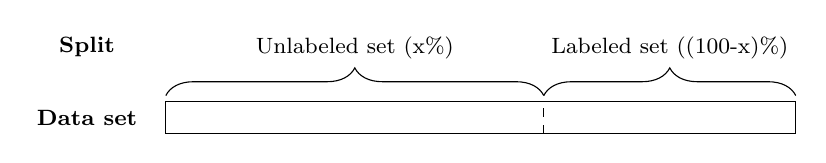
\begin{tikzpicture}[scale=0.8]
	\draw (0,0) rectangle (10,0.5) node[midway]{};
	\draw[dashed] (6,0) -- (6,0.5);
	
	\draw node[draw=none, xshift=-1cm, yshift=1.1cm, align=right] {\footnotesize \textbf{Split}};
	\draw node[draw=none, xshift=-1cm, yshift=.2cm] {\textbf{\footnotesize Data set}};
	
	\draw [decorate,decoration={brace,amplitude=10pt}, yshift=.1cm]
	(0,.5) -- (6,.5) node [black,midway,yshift=0.6cm] {\footnotesize Unlabeled set (x\%)};
	\draw [decorate,decoration={brace,amplitude=10pt}, yshift=.1cm]
	(6,.5) -- (10,.5) node [black,midway,yshift=0.6cm] {\footnotesize Labeled set ((100-x)\%)};
	
	\end{tikzpicture}
	\caption{The split-x process in specific data cases for graph-based models.}
	\label{fig3: data preparing process}
\end{figure}

Continue with similarity measure, there were 3 types of function in used including Euclidean, cosine and Gaussian kernel using default bandwidth equals to number of features. As graph sparsity methods are described in previous section \ref{section3: Graph Construction}, the experiments constructed three different kinds of graph with some modifies
\begin{description}
	\item[kNN graph:] Search for the most k similar vertices. The search range for k was $[1, 10]$. In the case of sparse graph, it is possible to have a component with all data that are unlabeled. We bypass this problem by constraining that there must be at least one labeled data in neighbor search.
	
	\item[MST tree:] Construct a maximum spanning tree on $\mathcal{G}$. The greedy Prim algorithm \parencite{6773228} was implemented. %The complexity of this algorithm is $\mathcal{O}(|E| log(n))$.
	
	\item[kNN-MST graph:] Construct a kNN graph first, then find a MST tree for each component of this kNN graph.
\end{description}

We only present the inference results of the mincut approach and graphical model using the influence index, we now short its name to the graphical model. The reason is that the conventional graphical model for our problem is not a completed one, it only works on a tree. Moreover, as has been shown in previous section, it does not have the adaption to our data assumption. Hence more or less, even with only the tree construction, it is no better than the mincut approach. Besides that, we have conducted the evaluation on the randomized mincut approach, section \ref{section3: mincut approach}, and it did not turn well either. The complete output of experiments and more details about the data resources and experiment reproduction are described in appendix \ref{appx: Experiments Resources}.

%%%%%%%%%%%%%%%%%%%%%%%%%%%%%%%%%%%%%%%%
\subsection{Semi-Supervised Evaluation}
\label{subsection: exp ssl}

The semi-supervised evaluation considers the ability of models to predict the unlabeled data in various scaling size of unlabeled set. The model learns all data instances and predicts the label for the unlabeled set. For each experimental data set, the experiment ran on 3 splits, split-70, split-90 and split-97, and the result was an average of 5-folds cross validation. In total we have 3 split sizes and 5-folds cross validation, $(3\times5) = 15$ evaluations for each model configuration.

\subsubsection*{Abalone and Digit data}
Abalone data was set on a binary task that determines the age range of abalone is $[5, 9]$ or $[10, 15]$ with 3842 instances, 7 features. The Digit data task was to clarify whether an $8\times8$ digit image, 64 features, is odd or even digit with 1797 instances. Both data were set on Euclidean similarity and Gaussian kernel with all three graph sparsity functions. Here we have 2 data cases, 2 similarity measurements, 3 graph types, $(2 \times 2 \times 3) = 12$ configurations. 

The experimental result of Abalone data using Euclidean similarity is in table \ref{table4: exp ssl abalone}, the trend is similar with Gaussian kernel. At first glance, we can observe that the mincut approach has the equivalent or better performance in case of split-70, especially with kNN graph. Here the kNN graph also illustrates its lead over MST and kNN-MST graphs. The situation changes when we significantly shrink the labeled size with split-97. Inform that the split-70 specifies that the unlabeled size is about 2 times bigger than the labeled one, while the split-97 means the difference is now about 32 times. In this case, the graphical model using kNN graph outperforms the mincut approach. Also the MST and kNN-MST graphs take off the gap with kNN graph and the results are nearly the same on both inference models.

We will continue with Digit data. In the same way, table \ref{table4: exp ssl digit} shows the results of Digit data with Euclidean similarity.  Take a look at graphical model, we may allegedly observe that, in kNN graph, the loopy propagation could not be converged on a group of vertices. This pushes the recall on positive label high up, but downgrades precision significantly compared with the mincut approach, and the reverse situation is applied to negative label. The equivalent outputs are held on MST and kNN-MST graph.

\subsubsection*{20Newsgroups data}
The 20Newsgroups data was constructed with tf-idf vectorization, the size of vocabulary reduced to 600 words by sum of tf-idf. The original data set consists of many groups of different topic labels. Here we set up an experiment between comp versus rec groups, in 8870 instances. We only use cosine similarity measurement with 3 types of graph construction. Thus we have 1 classifier, 1 similarity measurement, 3 graph types, $(1 \times 1 \times 3) = 3$ configurations.

The results are in table \ref{table4: exp ssl news}. This time, the performance of kNN graph prevails the other two graphs in both mincut approach and graphical model. With split-70 and split-90, we do not have much to say. But there in split-97, the mincut approach has fallen to a degenerate solution when vastly going for the negative label. If we solely examine the MST and kNN-MST graphs, the slightly better outcome comes from the mincut approach.  
% The situation is the same in comp versus sci task. Now we only examine the split-97 of this classifier in table \ref{table4: exp ssl news2 0.97}

%%%%%%%%%%%%%%%%%%%%%%%%%%%%%%%%%%%%%%%%
\subsection{Supervised Evaluation}
\label{subsection: exp sl}

In the same data setup of semi-supervised evaluation, for each data set, we plugin two supervised models including Logistic Regression and Support Vector Machines (SVM, using RBF kernel, $\gamma=\frac{1}{\#features}$) to predict the unlabeled data. In total we have 2 added supervised models, 3 split sizes and 5-folds cross validation, $(2 \times 3 \times 5) = 30$ additional evaluations for each data case. 

From the previous evaluation, we would claim the presume that with the carefully selected graph construction for a specific data, the graphical model can have the advantage over the mincut approach. Therefore, in this section, we only compare the supervised model with the graphical model. We also assume that we already evaluated the graph construction methods and utilize the best one here. 

In table \ref{table4: exp sl abalone} we have the comparison on Abalone data, the graphical model works on Euclidean kNN graph. The table starts with the split-70 where we have merely equivalent outcomes. Then go down with the split-90 and split-97, the logistic regression has the most recognizable downgrade. The graphical model has its solid performance and states first on split-97 in comparison with the other two. A similar result for Digit data is in table \ref{table4: exp sl digit} with Euclidean kNN-MST graph for graphical model. But at this time, the logistic regression has been downed from the beginning. Finally, the result of 20newsgroup data is in table \ref{table4: exp sl news}, graphical model utilizes cosine kNN graph. The supervised keeps its benefits in split-70 and split-90. In split-97, SVM has fallen into a degenerate trap when predicting most of the label for negative. It is the same situation with kNN graph of the mincut approach for this data case.

\pagebreak

\begin{table}[t!]
	\centering
	\captionsetup{justification=centering}
	\caption{Semi-supervised evaluation, Abalone data using Euclidean similarity.}
	\label{table4: exp ssl abalone}
	\makebox[\textwidth][c]{
		\begin{tabular}{ c|c|ccc|ccc }
			\multirow{2}{*}{Graph type} & \multirow{2}{*}{Label} & Precision & Recall & F1 & Precision & Recall & F1\\
			\cline{3-8}
			&& \multicolumn{3}{c}{\textbf{Mincut approach}} & \multicolumn{3}{c}{\textbf{Graphical model}} \\
			\hline
			
			\multicolumn{2}{c}{} & \multicolumn{6}{c}{Split-70, labeled:unlabeled = 1152:2690}\\
			
			\hline
			\multirow{3}{*}{kNN}
			& $-1$ & 0.73 & 0.79 & 0.76 & 0.69 & 0.79 & 0.73 \\
			& $+1$ & 0.80 & 0.74 & 0.76 & 0.78 & 0.67 & 0.72 \\
			\cline{2-8}
			& avg. & 0.76 & 0.76 & 0.76 & 0.74 & 0.73 & 0.73 \\
			\hline
			\multirow{3}{*}{MST} 
			& $-1$ & 0.72 & 0.71 & 0.71 & 0.72 & 0.71 & 0.71 \\
			& $+1$ & 0.74 & 0.75 & 0.74 & 0.74 & 0.75 & 0.74 \\
			\cline{2-8}
			& avg. & 0.73 & 0.73 & 0.73 & 0.73 & 0.73 & 0.73 \\
			\hline
			\multirow{3}{*}{kNN-MST} 
			& $-1$ & 0.71 & 0.70 & 0.70 & 0.71 & 0.70 & 0.70 \\
			& $+1$ & 0.73 & 0.75 & 0.74 & 0.73 & 0.75 & 0.74 \\
			\cline{2-8}
			& avg. & 0.72 & 0.72 & 0.72 & 0.72 & 0.72 & 0.72 \\
			\hline
			
			\multicolumn{2}{c}{} & \multicolumn{6}{c}{Split-90, labeled:unlabeled = 384:3458}\\
			
			\hline
			\multirow{3}{*}{kNN} 
			& $-1$ & 0.71 & 0.74 & 0.72 & 0.71 & 0.70 & 0.70 \\
			& $+1$ & 0.76 & 0.73 & 0.74 & 0.73 & 0.74 & 0.74 \\
			\cline{2-8}
			& avg. & 0.73 & 0.73 & 0.73 & 0.72 & 0.72 & 0.72 \\
			\hline
			\multirow{3}{*}{MST} 
			& $-1$ & 0.70 & 0.67 & 0.68 & 0.70 & 0.67 & 0.68 \\
			& $+1$ & 0.71 & 0.74 & 0.73 & 0.71 & 0.74 & 0.73 \\
			\cline{2-8}
			& avg. & 0.71 & 0.70 & 0.70 & 0.71 & 0.70 & 0.70 \\
			\hline
			\multirow{3}{*}{kNN-MST} 
			& $-1$ & 0.69 & 0.66 & 0.67 & 0.69 & 0.66 & 0.67 \\
			& $+1$ & 0.71 & 0.73 & 0.72  & 0.71 & 0.73 & 0.72 \\ 
			\cline{2-8}
			& avg. & 0.70 & 0.69 & 0.69 & 0.70 & 0.69 & 0.69 \\
			\hline
			
			\multicolumn{2}{c}{} & \multicolumn{6}{c}{Split-97, labeled:unlabeled = 115:3727}\\
			
			\hline
			\multirow{3}{*}{kNN} 
			& $-1$ & 0.69 & 0.66 & 0.67 & 0.69 & 0.73 & 0.71 \\
			& $+1$ & 0.70 & 0.73 & 0.72 & 0.74 & 0.71 & 0.72 \\
			\cline{2-8}
			& avg. & 0.69 & 0.69 & 0.69 & 0.72 & 0.72 & 0.72 \\
			\hline
			\multirow{3}{*}{MST} 
			& $-1$ & 0.70 & 0.64 & 0.67 & 0.70 & 0.64 & 0.67 \\
			& $+1$ & 0.70 & 0.75 & 0.72 & 0.70 & 0.75 & 0.72 \\
			\cline{2-8}
			& avg. & 0.70 & 0.70 & 0.70 & 0.70 & 0.70 & 0.70 \\
			\hline
			\multirow{3}{*}{kNN-MST} 
			& $-1$ & 0.69 & 0.64 & 0.66 & 0.69 & 0.64 & 0.66 \\
			& $+1$ & 0.70 & 0.73 & 0.71 & 0.70 & 0.73 & 0.71 \\
			\cline{2-8}
			& avg. & 0.69 & 0.69 & 0.69 & 0.69 & 0.69 & 0.69 \\
			\hline
	\end{tabular}}
\end{table}

\begin{table}[t!]
	\centering
	\captionsetup{justification=centering}
	\caption{Semi-supervised evaluation, Digit data using Euclidean similarity.}
	\label{table4: exp ssl digit}
	\makebox[\textwidth][c]{
		\begin{tabular}{ c|c|ccc|ccc }
			\multirow{2}{*}{Graph type} & \multirow{2}{*}{Label} & Precision & Recall & F1 & Precision & Recall & F1\\
			\cline{3-8}
			&& \multicolumn{3}{c}{\textbf{Mincut approach}} & \multicolumn{3}{c}{\textbf{Graphical model}} \\
			\hline
			
			\multicolumn{2}{c}{} & \multicolumn{6}{c}{Split-70,  data number labeled-unlabeled : 539-1258}\\
			
			\hline
			\multirow{3}{*}{kNN} 
			& $-1$ & 1.00 & 0.99 & 0.99 & 1.00 & 0.99 & 0.99 \\
			& $+1$ & 0.99 & 1.00 & 0.99 & 0.99 & 1.00 & 0.99 \\
			\cline{2-8}
			& avg. & 0.99 & 0.99 & 0.99 & 0.99 & 0.99 & 0.99 \\
			\hline
			\multirow{3}{*}{MST} 
			& $-1$ & 1.00 & 0.99 & 0.99 & 1.00 & 0.99 & 0.99 \\
			& $+1$ & 0.99 & 1.00 & 0.99 & 0.99 & 1.00 & 0.99 \\
			\cline{2-8}
			& avg. & 0.99 & 0.99 & 0.99 & 0.99 & 0.99 & 0.99 \\
			\hline
			\multirow{3}{*}{kNN-MST} 
			& $-1$ & 1.00 & 0.99 & 0.99 & 1.00 & 0.99 & 0.99 \\
			& $+1$ & 0.99 & 1.00 & 0.99 & 0.99 & 1.00 & 0.99 \\
			\cline{2-8}
			& avg. & 0.99 & 0.99 & 0.99 & 0.99 & 0.99 & 0.99 \\
			\hline
			
			\multicolumn{2}{c}{} & \multicolumn{6}{c}{Split-90,  data number labeled-unlabeled : 179-1618}\\
			
			\hline
			\multirow{3}{*}{kNN} 
			& $-1$ & 0.98 & 0.98 & 0.98 & 0.93 & 0.84 & 0.88 \\
			& $+1$ & 0.98 & 0.98 & 0.98 & 0.86 & 0.94 & 0.90 \\
			\cline{2-8}
			& avg. & 0.98 & 0.98 & 0.98 & 0.89 & 0.89 & 0.89 \\
			\hline
			\multirow{3}{*}{MST} 
			& $-1$ & 0.99 & 0.98 & 0.99 & 0.99 & 0.98 & 0.99 \\
			& $+1$ & 0.99 & 0.99 & 0.99 & 0.99 & 0.99 & 0.99 \\
			\cline{2-8}
			& avg. & 0.99 & 0.99 & 0.99 & 0.99 & 0.99 & 0.99 \\
			\hline
			\multirow{3}{*}{kNN-MST} 
			& $-1$ & 0.99 & 0.98 & 0.99 & 0.99 & 0.98 & 0.99 \\
			& $+1$ & 0.98 & 0.99 & 0.99 & 0.98 & 0.99 & 0.99 \\ 
			\cline{2-8}
			& avg. & 0.99 & 0.99 & 0.99 & 0.99 & 0.99 & 0.99 \\
			\hline
			
			\multicolumn{2}{c}{} & \multicolumn{6}{c}{Split-97,  data number labeled-unlabeled : 53-1744}\\
			
			\hline
			\multirow{3}{*}{kNN} 
			& $-1$ & 0.93 & 0.97 & 0.95 & 0.91 & 0.77 & 0.83 \\
			& $+1$ & 0.97 & 0.93 & 0.95 & 0.80 & 0.92 & 0.86 \\
			\cline{2-8}
			& avg. & 0.95 & 0.95 & 0.95 & 0.86 & 0.84 & 0.84 \\
			\hline
			\multirow{3}{*}{MST} 
			& $-1$ & 0.90 & 0.98 & 0.93 & 0.90 & 0.98 & 0.93 \\
			& $+1$ & 0.98 & 0.88 & 0.93 & 0.98 & 0.88 & 0.93 \\
			\cline{2-8}
			& avg. & 0.94 & 0.93 & 0.93 & 0.94 & 0.93 & 0.93 \\
			\hline
			\multirow{3}{*}{kNN-MST} 
			& $-1$ & 0.94 & 0.96 & 0.95 & 0.94 & 0.96 & 0.95 \\
			& $+1$ & 0.96 & 0.94 & 0.95 & 0.96 & 0.94 & 0.95 \\
			\cline{2-8}
			& avg. & 0.95 & 0.95 & 0.95 & 0.95 & 0.95 & 0.95 \\
			\hline
	\end{tabular}}
\end{table}

\begin{table}[t!]
	\centering
	\captionsetup{justification=centering}
	\caption{Semi-supervised evaluation, 20Newsgroups data, comp versus rec using cosine similarity.}
	\label{table4: exp ssl news}
	\makebox[\textwidth][c]{
		\begin{tabular}{ c|c|ccc|ccc }
			\multirow{2}{*}{Graph type} & \multirow{2}{*}{Label} & Precision & Recall & F1 & Precision & Recall & F1\\
			\cline{3-8}
			&& \multicolumn{3}{c}{\textbf{Mincut approach}} & \multicolumn{3}{c}{\textbf{Graphical model}} \\
			\hline
			
			\multicolumn{2}{c}{} & \multicolumn{6}{c}{Split-70, labeled:unlabeled = 2661:6209}\\
			
			\hline
			\multirow{3}{*}{kNN}
			& $-1$ & 0.89 & 0.84 & 0.86 & 0.82 & 0.96 & 0.88 \\
			& $+1$ & 0.81 & 0.88 & 0.84 & 0.94 & 0.73 & 0.82 \\
			\cline{2-8}
			& avg. & 0.85 & 0.86 & 0.85 & 0.88 & 0.85 & 0.85 \\ 
			\hline
			\multirow{3}{*}{MST} 
			& $-1$ & 0.86 & 0.80 & 0.83 & 0.82 & 0.83 & 0.83 \\
			& $+1$ & 0.77 & 0.84 & 0.81 & 0.79 & 0.78 & 0.79 \\
			\cline{2-8}
			& avg. & 0.82 & 0.82 & 0.82 & 0.81 & 0.81 & 0.81 \\
			\hline
			\multirow{3}{*}{kNN-MST} 
			& $-1$ & 0.86 & 0.80 & 0.83 & 0.82 & 0.83 & 0.83 \\
			& $+1$ & 0.78 & 0.84 & 0.81 & 0.79 & 0.78 & 0.79 \\
			\cline{2-8}
			& avg. & 0.82 & 0.82 & 0.82 & 0.81 & 0.81 & 0.81 \\
			\hline
			
			\multicolumn{2}{c}{} & \multicolumn{6}{c}{Split-90, labeled:unlabeled = 860:8010 }\\
			
			\hline
			\multirow{3}{*}{kNN}
			& $-1$ & 0.91 & 0.82 & 0.86 & 0.80 & 0.96 & 0.88 \\
			& $+1$ & 0.80 & 0.89 & 0.85 & 0.94 & 0.71 & 0.81 \\
			\cline{2-8}
			& avg. & 0.85 & 0.86 & 0.85 & 0.87 & 0.84 & 0.84 \\
			\hline
			\multirow{3}{*}{MST} 
			& $-1$ & 0.82 & 0.78 & 0.80 & 0.79 & 0.82 & 0.80 \\
			& $+1$ & 0.75 & 0.79 & 0.77 & 0.77 & 0.73 & 0.75 \\
			\cline{2-8}
			& avg. & 0.79 & 0.79 & 0.79 & 0.78 & 0.77 & 0.78 \\
			\hline
			\multirow{3}{*}{kNN-MST} 
			& $-1$ & 0.84 & 0.80 & 0.82 & 0.80 & 0.83 & 0.82 \\
			& $+1$ & 0.77 & 0.81 & 0.79 & 0.78 & 0.75 & 0.77 \\
			\cline{2-8}
			& avg. & 0.80 & 0.80 & 0.80 & 0.79 & 0.79 & 0.79 \\
			\hline
			
			\multicolumn{2}{c}{} & \multicolumn{6}{c}{Split-97, labeled:unlabeled = 266:8604}\\
			
			\hline
			\multirow{3}{*}{kNN} 
			& $-1$ & 0.56 & 0.97 & 0.71 & 0.82 & 0.94 & 0.87 \\
			& $+1$ & 0.59 & 0.06 & 0.11 & 0.91 & 0.74 & 0.81 \\
			\cline{2-8}
			& avg. & 0.57 & 0.51 & 0.41 & 0.86 & 0.84 & 0.84 \\
			\hline
			\multirow{3}{*}{MST} 
			& $-1$ & 0.80 & 0.77 & 0.79 & 0.77 & 0.81 & 0.79 \\
			& $+1$ & 0.73 & 0.77 & 0.75 & 0.75 & 0.70 & 0.73 \\
			\cline{2-8}
			& avg. & 0.77 & 0.77 & 0.77 & 0.76 & 0.76 & 0.76 \\
			\hline
			\multirow{3}{*}{kNN-MST} 
			& $-1$ & 0.81 & 0.79 & 0.80 & 0.78 & 0.82 & 0.80 \\
			& $+1$ & 0.75 & 0.78 & 0.76 & 0.77 & 0.72 & 0.74 \\
			\cline{2-8}
			& avg. & 0.78 & 0.78 & 0.78 & 0.77 & 0.77 & 0.77 \\
			\hline
			
	\end{tabular}}
\end{table}

\begin{table}[t!]
	\centering
	\captionsetup{justification=centering}
	\caption{Supervised evaluation, Abalone data.}
	\makebox[\textwidth][c]{
		\begin{tabular}{ c|ccc|ccc|ccc }
			\multirow{2}{*}{Label} & Precision & Recall & F1 & Precision & Recall & F1 & Precision & Recall & F1\\
			\cline{2-10}
			& \multicolumn{3}{c}{\textbf{Logistic Regression}} & \multicolumn{3}{c}{\textbf{SVM}} & \multicolumn{3}{c}{\textbf{Graphical model}} \\
			\hline
			
			\multicolumn{1}{c}{} & \multicolumn{9}{c}{Split-70} \\
			\hline
			$-1$ & 0.72 & 0.73 & 0.72 & 0.69 & 0.78 & 0.73 & 0.69 & 0.79 & 0.73 \\
			$+1$ & 0.75 & 0.75 & 0.75 & 0.78 & 0.68 & 0.72 & 0.78 & 0.67 & 0.72 \\
			\cline{1-10}
			avg. & 0.74 & 0.74 & 0.74 & 0.73 & 0.73 & 0.73 & 0.74 & 0.73 & 0.73 \\
			\hline
			
			\multicolumn{1}{c}{} & \multicolumn{9}{c}{Split-90} \\
			\hline
			$-1$ & 0.71 & 0.62 & 0.66 & 0.69 & 0.74 & 0.71 & 0.71 & 0.70 & 0.70 \\
			$+1$ & 0.69 & 0.77 & 0.73 & 0.75 & 0.70 & 0.72 & 0.73 & 0.74 & 0.74 \\
			\cline{1-10}
			avg. & 0.70 & 0.69 & 0.69 & 0.72 & 0.72 & 0.72 & 0.72 & 0.72 & 0.72 \\
			\hline
			
			\multicolumn{1}{c}{} & \multicolumn{9}{c}{Split-97} \\
			\hline
			$-1$ & 0.70 & 0.65 & 0.67 & 0.66 & 0.79 & 0.72 & 0.69 & 0.73 & 0.71 \\
			$+1$ & 0.71 & 0.74 & 0.72 & 0.78 & 0.63 & 0.69 & 0.74 & 0.71 & 0.72 \\
			\cline{1-10}
			avg. & 0.70 & 0.70 & 0.69 & 0.72 & 0.71 & 0.70 & 0.72 & 0.72 & 0.72 \\
			\hline
	\end{tabular}}
	\label{table4: exp sl abalone}
\end{table}

\begin{table}[t!]
	\centering
	\captionsetup{justification=centering}
	\caption{Supervised evaluation, Digit data.}
	\makebox[\textwidth][c]{
		\begin{tabular}{ c|ccc|ccc|ccc }
			\multirow{2}{*}{Label} & Precision & Recall & F1 & Precision & Recall & F1 & Precision & Recall & F1\\
			\cline{2-10}
			& \multicolumn{3}{c}{\textbf{Logistic Regression}} & \multicolumn{3}{c}{\textbf{SVM}} & \multicolumn{3}{c}{\textbf{Graphical model}} \\
			\hline
			
			\multicolumn{1}{c}{} & \multicolumn{9}{c}{Split-70} \\
			\hline
			$-1$ & 0.90 & 0.89 & 0.90 & 1.00 & 0.98 & 0.99 & 1.00 & 0.99 & 0.99 \\
			$+1$ & 0.90 & 0.91 & 0.90 & 0.98 & 1.00 & 0.99 & 0.99 & 1.00 & 0.99 \\
			\cline{1-10}
			avg. & 0.90 & 0.90 & 0.90 & 0.99 & 0.99 & 0.99 & 0.99 & 0.99 & 0.99 \\
			\hline
			
			\multicolumn{1}{c}{} & \multicolumn{9}{c}{Split-90} \\
			\hline
			$-1$ & 0.88 & 0.86 & 0.87 & 0.98 & 0.95 & 0.97 & 0.99 & 0.98 & 0.99 \\
			$+1$ & 0.87 & 0.88 & 0.88 & 0.96 & 0.98 & 0.97 & 0.98 & 0.99 & 0.99 \\
			\cline{1-10}
			avg. & 0.87 & 0.87 & 0.87 & 0.97 & 0.97 & 0.97 & 0.99 & 0.99 & 0.99 \\
			\hline
			
			\multicolumn{1}{c}{} & \multicolumn{9}{c}{Split-97} \\
			\hline
			$-1$ & 0.83 & 0.82 & 0.82 & 0.94 & 0.88 & 0.90 & 0.94 & 0.96 & 0.95 \\
			$+1$ & 0.83 & 0.83 & 0.83 & 0.89 & 0.94 & 0.91 & 0.96 & 0.94 & 0.95 \\
			\cline{1-10}
			avg. & 0.83 & 0.83 & 0.83 & 0.91 & 0.91 & 0.91 & 0.95 & 0.95 & 0.95 \\
			\hline
	\end{tabular}}
	\label{table4: exp sl digit}
\end{table}

\begin{table}[t!]
	\centering
	\captionsetup{justification=centering}
	\caption{Supervised evaluation, 20Newsgroups data, comp versus rec.}
	\makebox[\textwidth][c]{
		\begin{tabular}{ c|ccc|ccc|ccc }
			\multirow{2}{*}{Label} & Precision & Recall & F1 & Precision & Recall & F1 & Precision & Recall & F1\\
			\cline{2-10}
			& \multicolumn{3}{c}{\textbf{Logistic Regression}} & \multicolumn{3}{c}{\textbf{SVM}} & \multicolumn{3}{c}{\textbf{Graphical model}} \\
			\hline
			
			\multicolumn{1}{c}{} & \multicolumn{9}{c}{Split-70} \\
			\hline
			$-1$ & 0.92 & 0.89 & 0.90 & 0.90 & 0.90 & 0.90 & 0.82 & 0.96 & 0.88 \\
			$+1$ & 0.87 & 0.90 & 0.89 & 0.87 & 0.88 & 0.88 & 0.94 & 0.73 & 0.82 \\
			\cline{1-10}
			avg. & 0.89 & 0.90 & 0.90 & 0.89 & 0.89 & 0.89 & 0.88 & 0.85 & 0.85 \\
			\hline
			
			\multicolumn{1}{c}{} & \multicolumn{9}{c}{Split-90} \\
			\hline
			$-1$ & 0.90 & 0.90 & 0.90 & 0.79 & 0.97 & 0.87 & 0.80 & 0.96 & 0.88 \\
			$+1$ & 0.88 & 0.88 & 0.88 & 0.95 & 0.68 & 0.79 & 0.94 & 0.71 & 0.81 \\
			\cline{1-10}
			avg. & 0.89 & 0.89 & 0.89 & 0.87 & 0.82 & 0.83 & 0.87 & 0.84 & 0.84 \\
			\hline
			
			\multicolumn{1}{c}{} & \multicolumn{9}{c}{Split-97} \\
			\hline
			$-1$ & 0.82 & 0.93 & 0.87 & 0.55 & 1.00 & 0.71 & 0.82 & 0.94 & 0.87 \\
			$+1$ & 0.90 & 0.74 & 0.81 & 1.00 & 0.01 & 0.01 & 0.91 & 0.74 & 0.81 \\
			\cline{1-10}
			avg. & 0.86 & 0.84 & 0.84 & 0.78 & 0.50 & 0.36 & 0.86 & 0.84 & 0.84 \\
			\hline
	\end{tabular}}
	\label{table4: exp sl news}
\end{table}